\subsection{Neural Network Design and Training}
\label{subsec:nntraining}

%\begin{wrapfigure}{r}{0.5\textwidth}
%	\centering
%    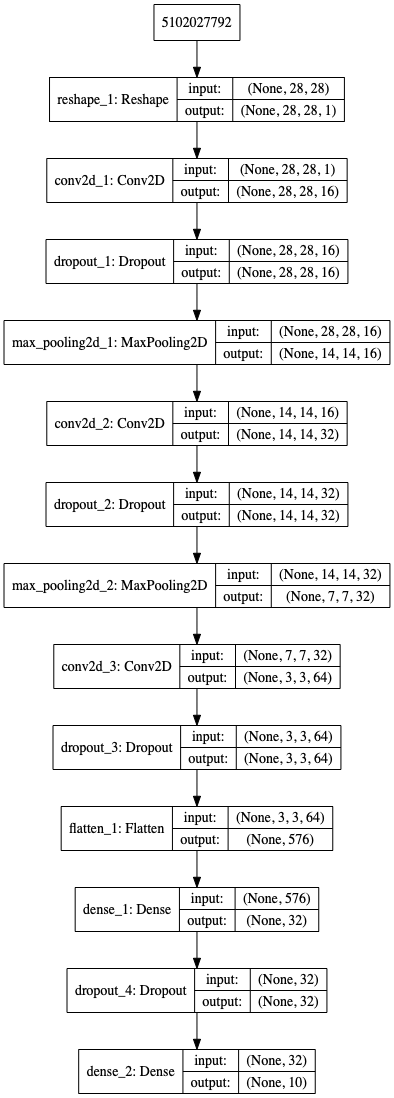
\includegraphics[width=0.35\textwidth]{img/nnlayout}
%	\caption{Network Layers}
%	\label{fig:network-layers}
%\end{wrapfigure}


The network was implemented in PyTorch \cite{Paszke:2019aa} as well as Tensorflow \cite{MartinAbadi:2015aa}. The backend was later exclusively switched to PyTorch (which is also the most common deep learning framework in Science) due to its better support of quantization. The layers of the neural network are depicted in Figure~\ref{fig:eggnet}. 
The network was trained on the \emph{MNIST} dataset which consists of 60.000 images of handwritten digits. Those where split up in 50.000 images used for training and 10.000 used for evaluation. The network maps mathematically an $28 \times 28$ input image $x \in \mathbb{R}^{28,28}$ to an output of vector of probabilities $y \in \mathbb{R}^{10}$ where each value corresponds how likely the input image belongs to that class. The layers of the network are listed in Table~\ref{tab:eggnet-layers}.

\begin{table}[h]
	\centering
	\begin{tabular}{clcl}
		\toprule
		Layer & Type	& 	Data Size (output)	& Purpose \\
		\midrule
		 1 & Conv01		&	$[28,28,16]$	& Extract features ($[3,3]$ kernels)		  \\
		 2 & ReLU		&	$[28,28,16]$	& Introduce nonlinearity  \\
		 3 & Pool01		&	$[14,14,16]$	& Introduce nonlinearity, reduce dimensions  \\
		 4 & Conv02 	&	$[14,14,32]$	& Extract features 	($[3,3]$ kernels)	  \\
		 5 & ReLU		&	$[14,14,32]$	& Introduce nonlinearity  \\
		 6 & Pool02		&	$[7,7,32]$	& Introduce nonlinearity, reduce dimensions  \\
		 7 & Dense01	&	$[32]$		& Combine features  \\
		 8 & ReLU		&	$[32]$		& Introduce nonlinearity  \\
		 9 & Dense02	&	$[10]$		& Combine features  \\
		10 & Softmax 	&	$[10]$		& Normalize output  \\
		\bottomrule
	\end{tabular}
	\caption{Eggnet Layers}
	\label{tab:eggnet-layers}
\end{table}

Further for training of the network the \emph{ADAM} optimization algorithm \cite{Kingma:2014aa} was used to minimize the cross-entropy-loss function which is defined as
\begin{equation}
    J = - y  \log(h) + (1-y)  \log(1-h)
\end{equation}
This loss function is standard for classification problems where each sample belongs to exactly one class. 
The ADAM algorithm can be adjusted by parameters, which control the speed of convergence. The recommended values, listed in Table~\ref{tab:train-params}, by \cite{Kingma:2014aa} were used.
\begin{table}[ht]
	\centering
    \begin{tabular}{cc}
        \toprule
            Parameter & Value \\
        \midrule
            $\alpha$   & $0.001$ \\
            $\beta_1$  & $0.9$   \\
            $\beta_2$  & $0.999$  \\          
        \bottomrule
    \end{tabular}
    \caption{Network Training Parameters}
    \label{tab:train-params}
\end{table}


A useful guide for implementing convolutions can be found in \cite{dumoulin2016guide}. The training of the network yielded very high accuracy rates that are typical for the MNIST dataset, which is an easy challenge for machine learning. Even though the network performance could be improved, e.g. by hyperparameter tuning the results were acceptable for our case. The progress of the training in terms of accuracy and loss can be seen in Figure~\ref{fig:network-train-acc} respectively in Figure~\ref{fig:network-train-loss}. The final output of the network over the training is evaluated in Figure~\ref{fig:network-test-cm} for real values and in Figure~\ref{fig:network-test-qcm} for fake quantized values.

Both, PyTorch and Tensorflow/Keras are Python libraries but most \gls{acr:NN} operations are not implemented in Python directly because of performance reasons. This makes debugging more difficult which is why we reimplemented the operations we needed in Python. This was done using NumPy and SWIG, which will be discussed more extensively in Section~\ref{sec:sw-python}, and enabled us to verify the correct ordering of parameters, weights and activations.

\begin{figure}[hbtp]
\centering
\begin{subfigure}[t]{0.5\textwidth}
	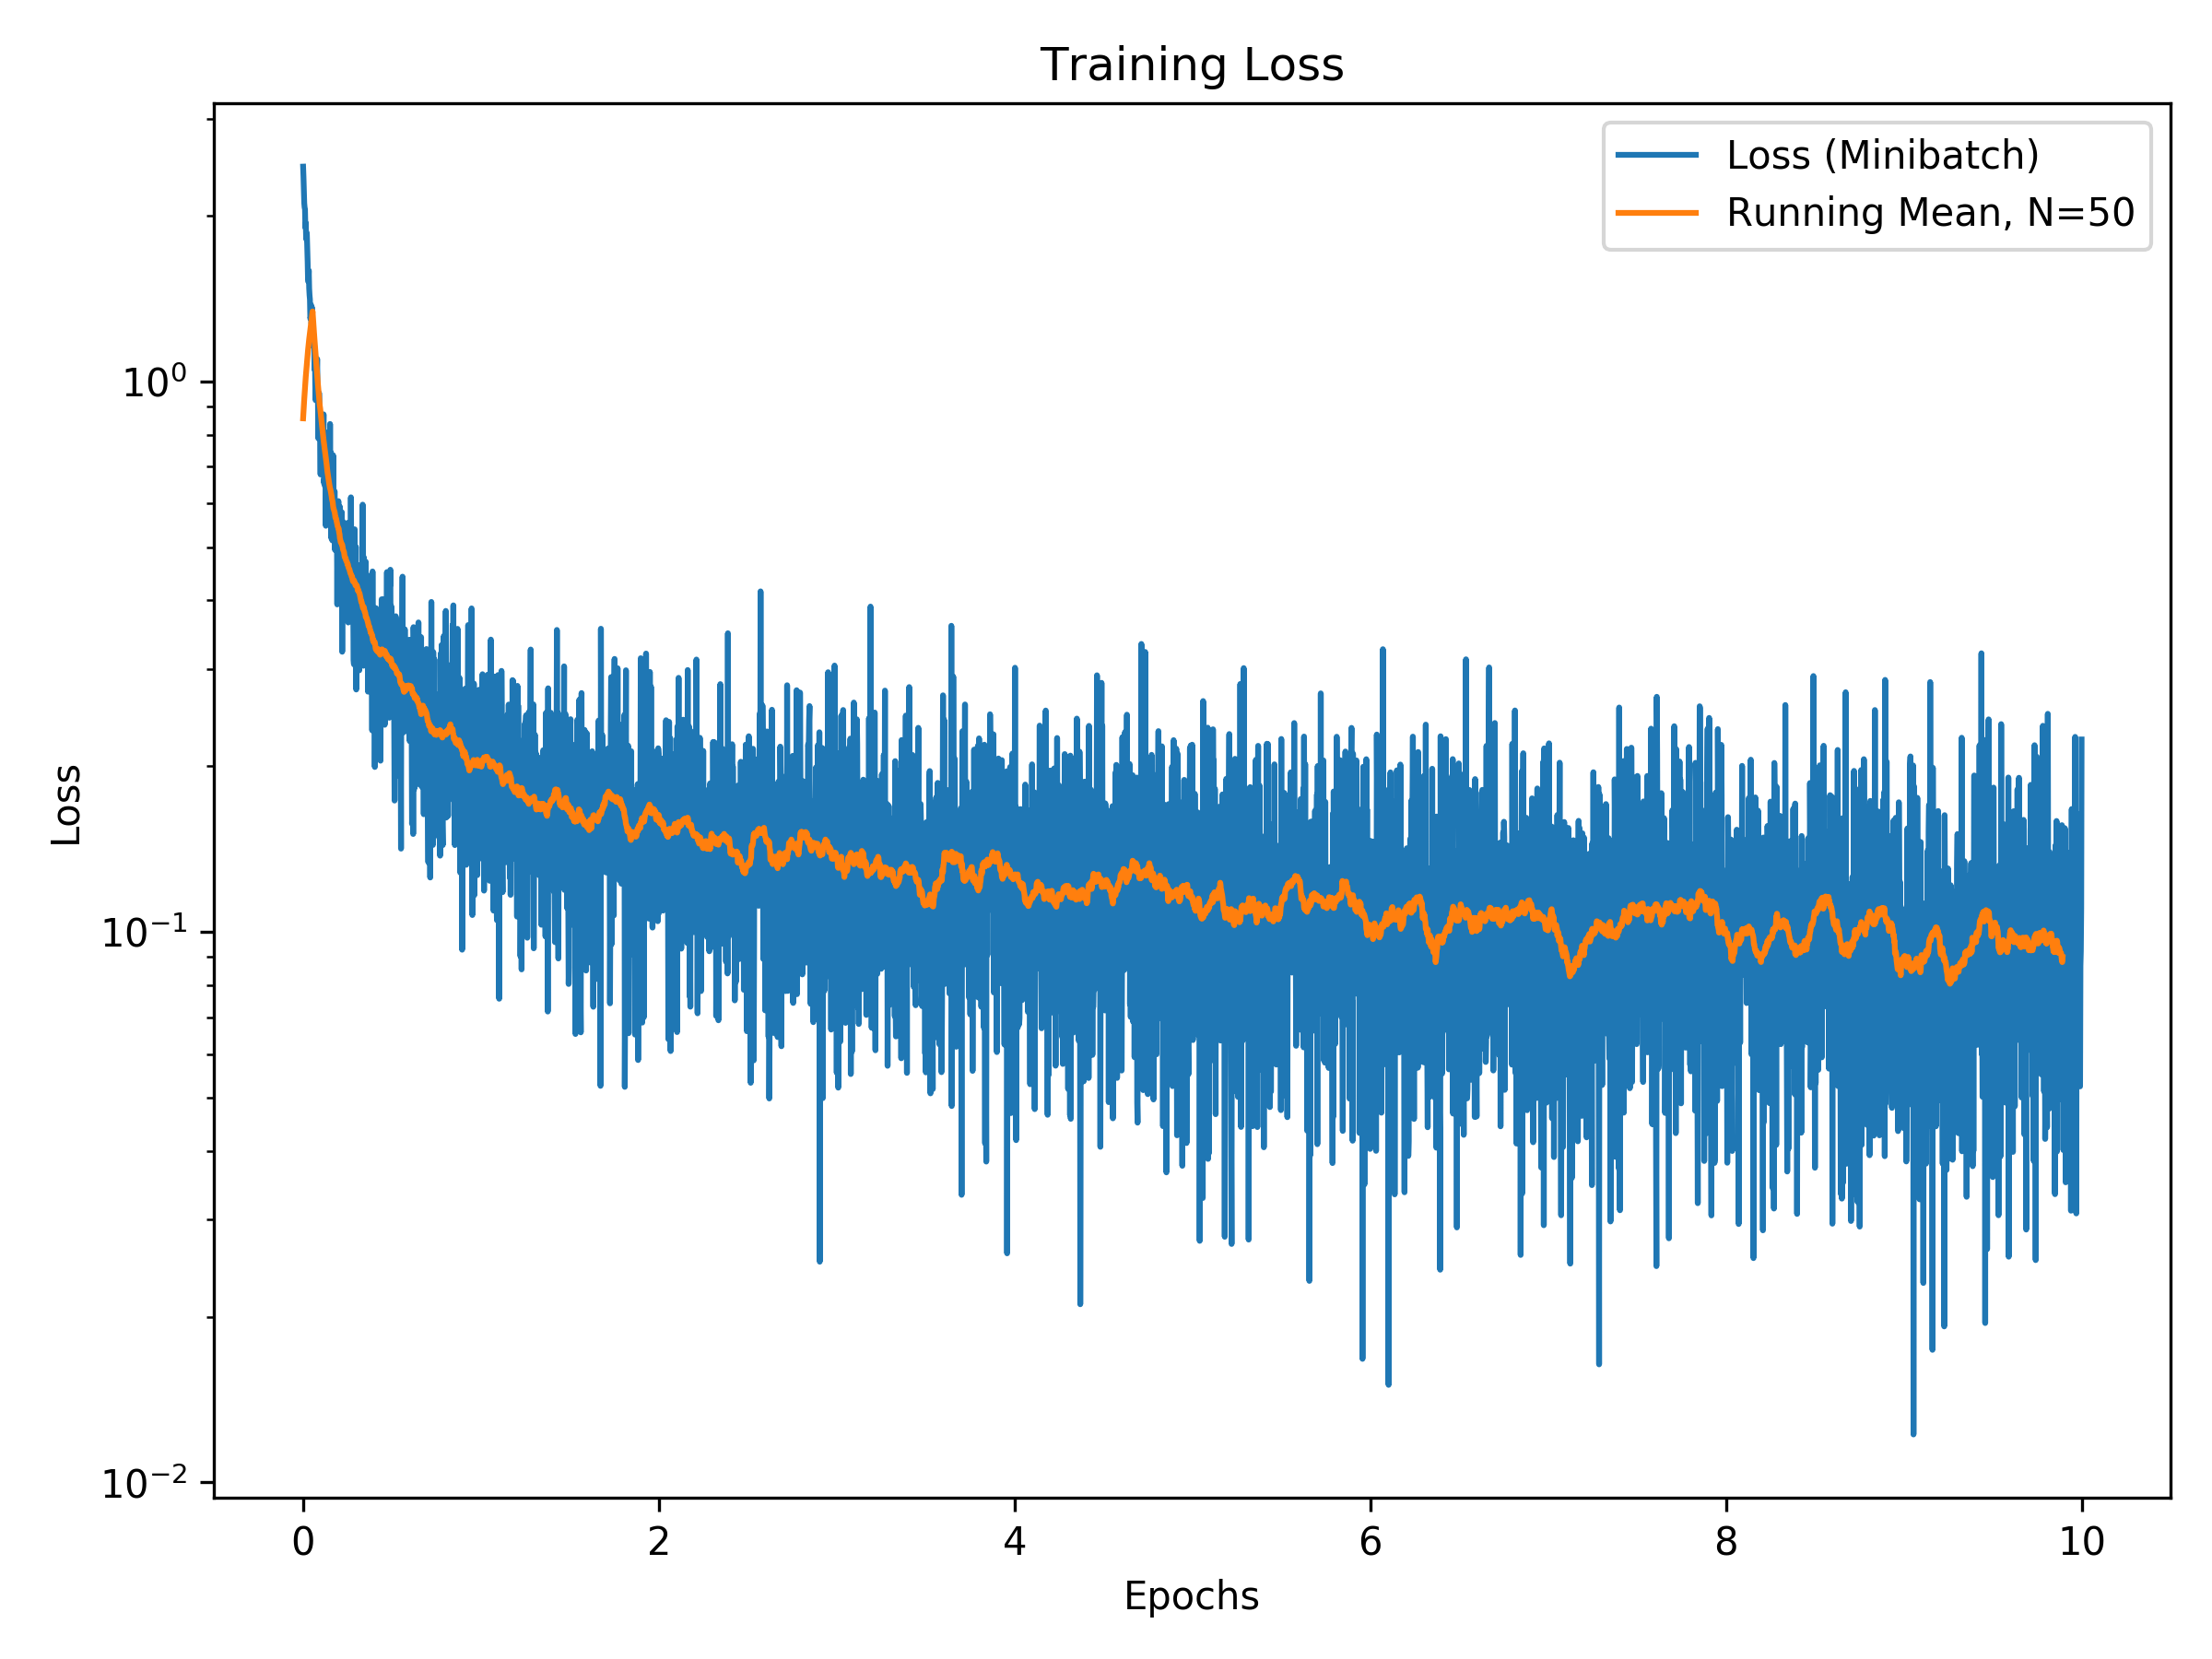
\includegraphics[width=0.8\textwidth]{../../net/images/training_loss}
	\caption{Training Loss}		
	\label{fig:network-train-loss}
\end{subfigure}%
~
\begin{subfigure}[t]{0.5\textwidth}
	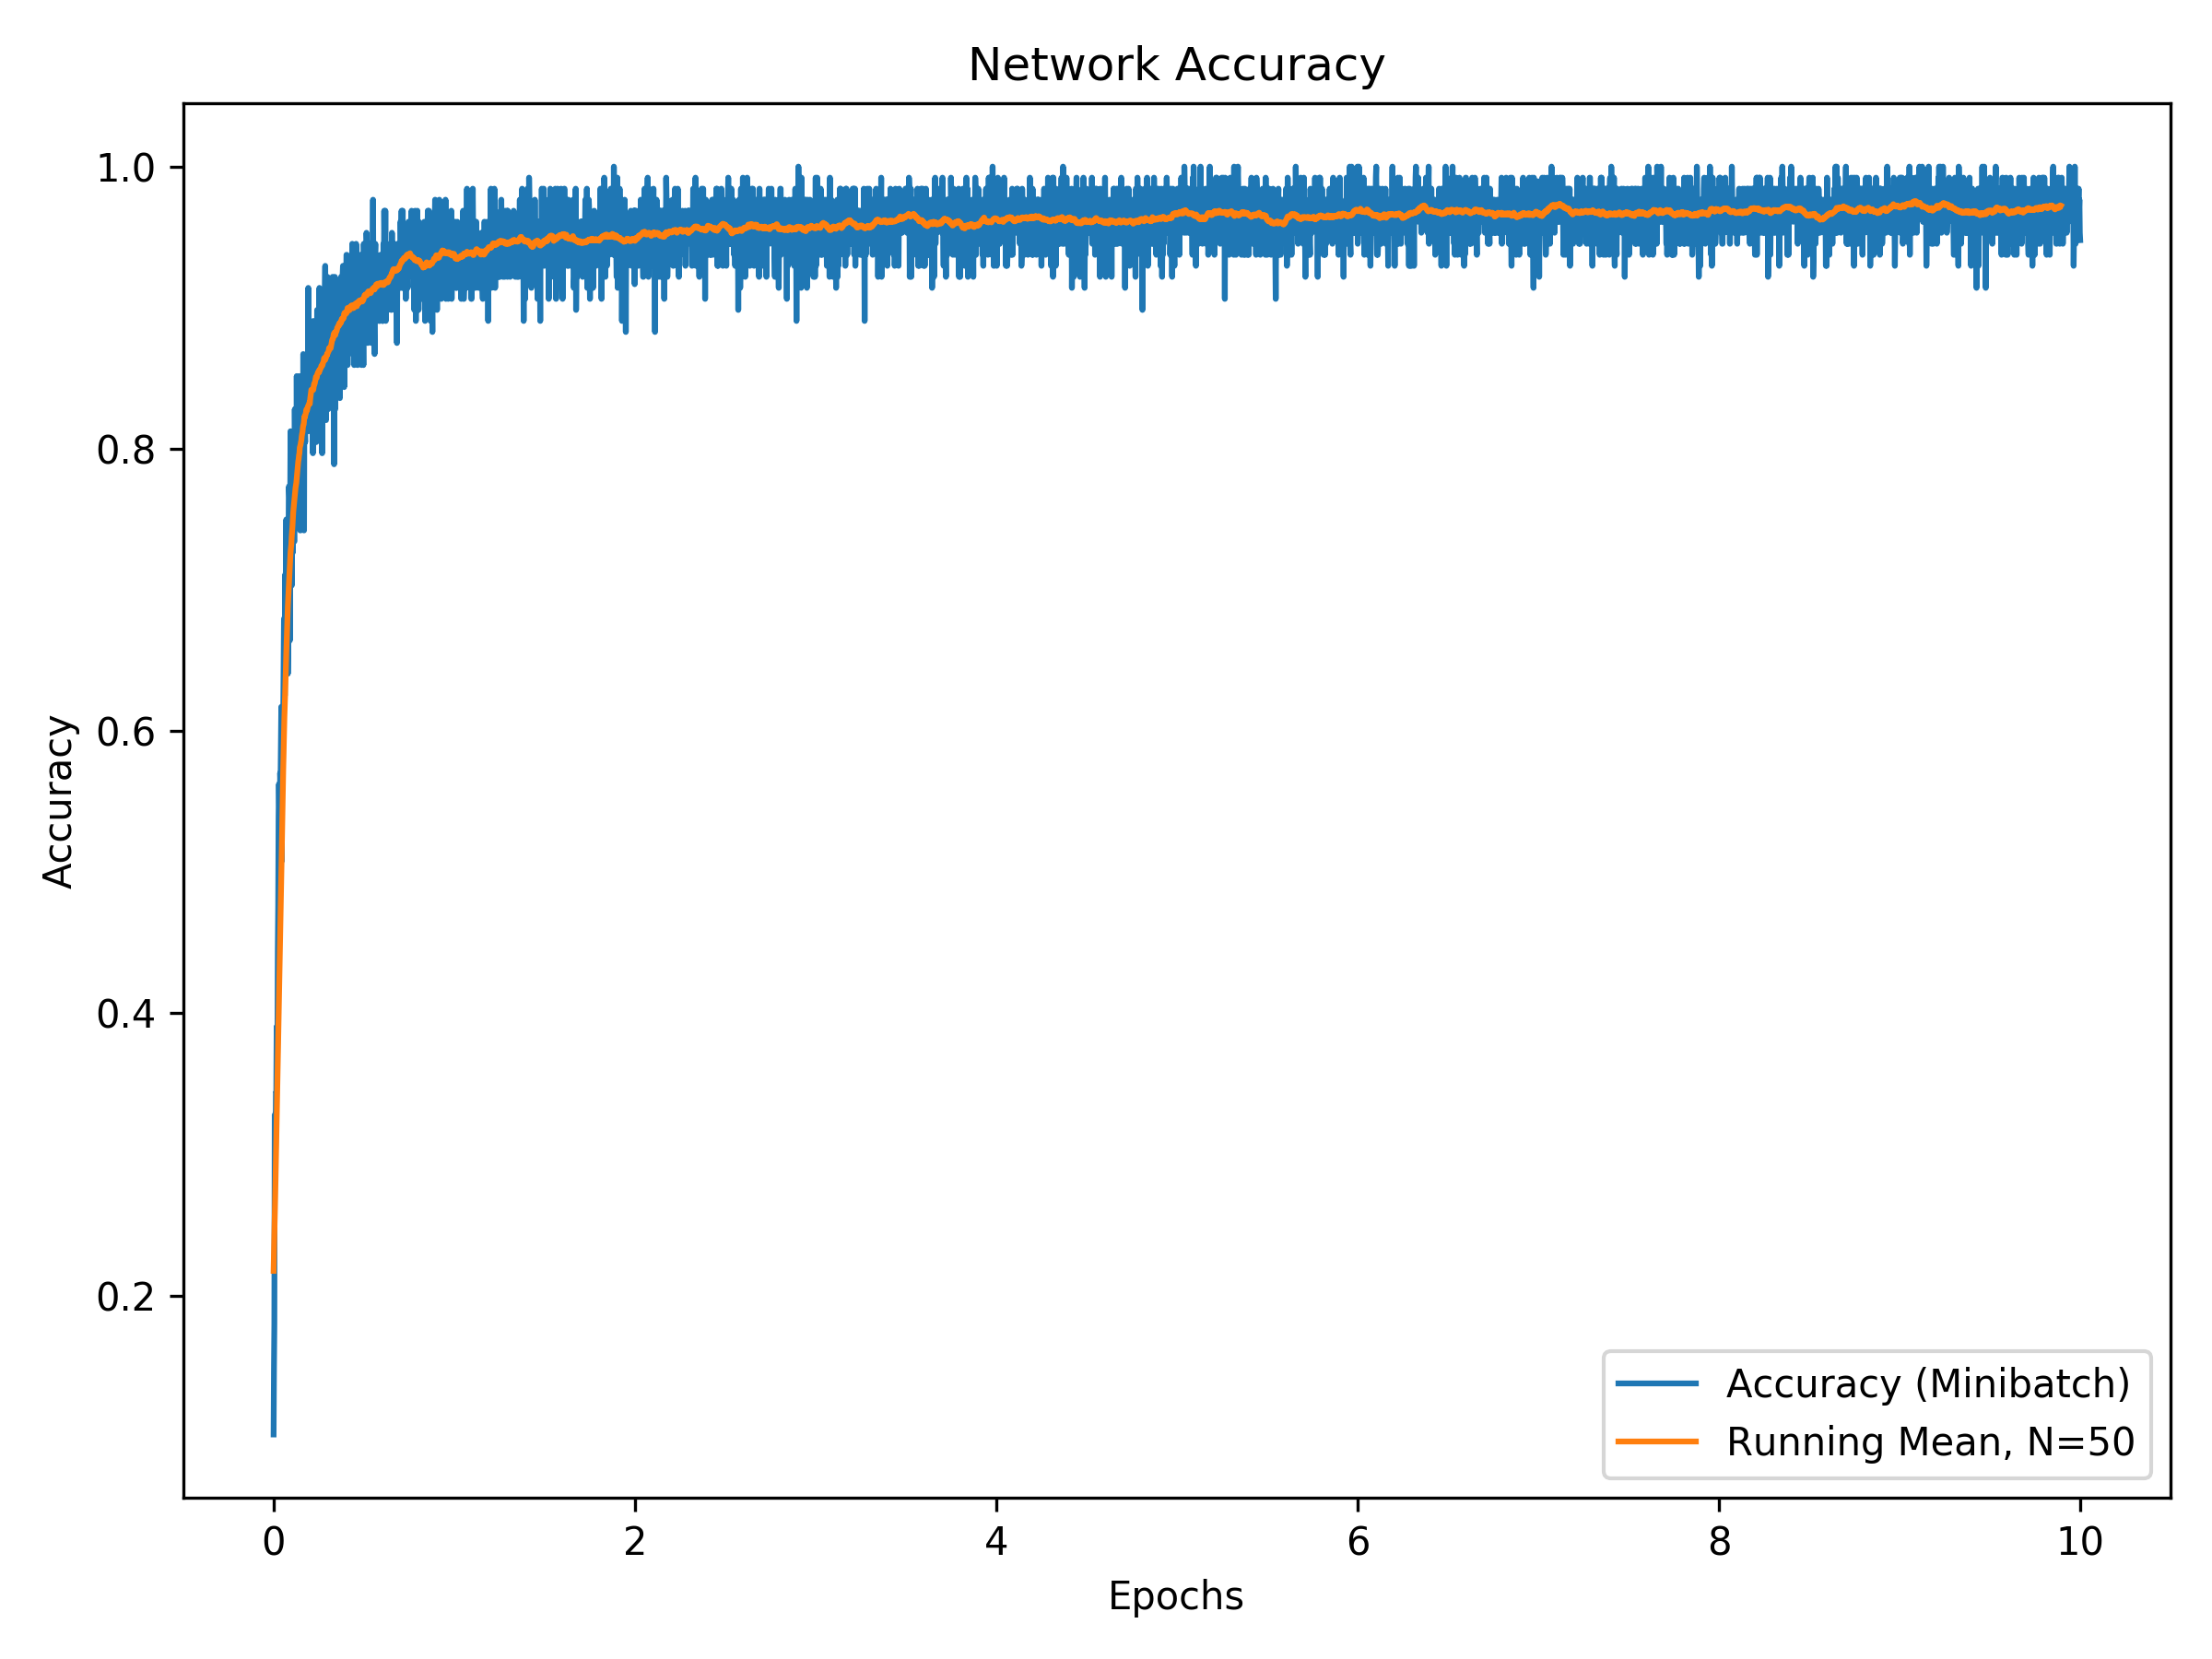
\includegraphics[width=0.8\textwidth]{../../net/images/training_accuracy}
	\caption{Training Accuracy}
	\label{fig:network-train-acc}		
\end{subfigure}
\caption[Network loss and accuracy over the training iterations]{Network loss and accuracy over the training iterations. The blue lines show spikes which occur because of the randomly selected mini batches. The orange line shows the smoothed version over 50 periods}
\label{fig:network-training-graphs}
\end{figure}

\begin{figure}[hbtp]
\centering
\begin{subfigure}[t]{0.5\textwidth}
	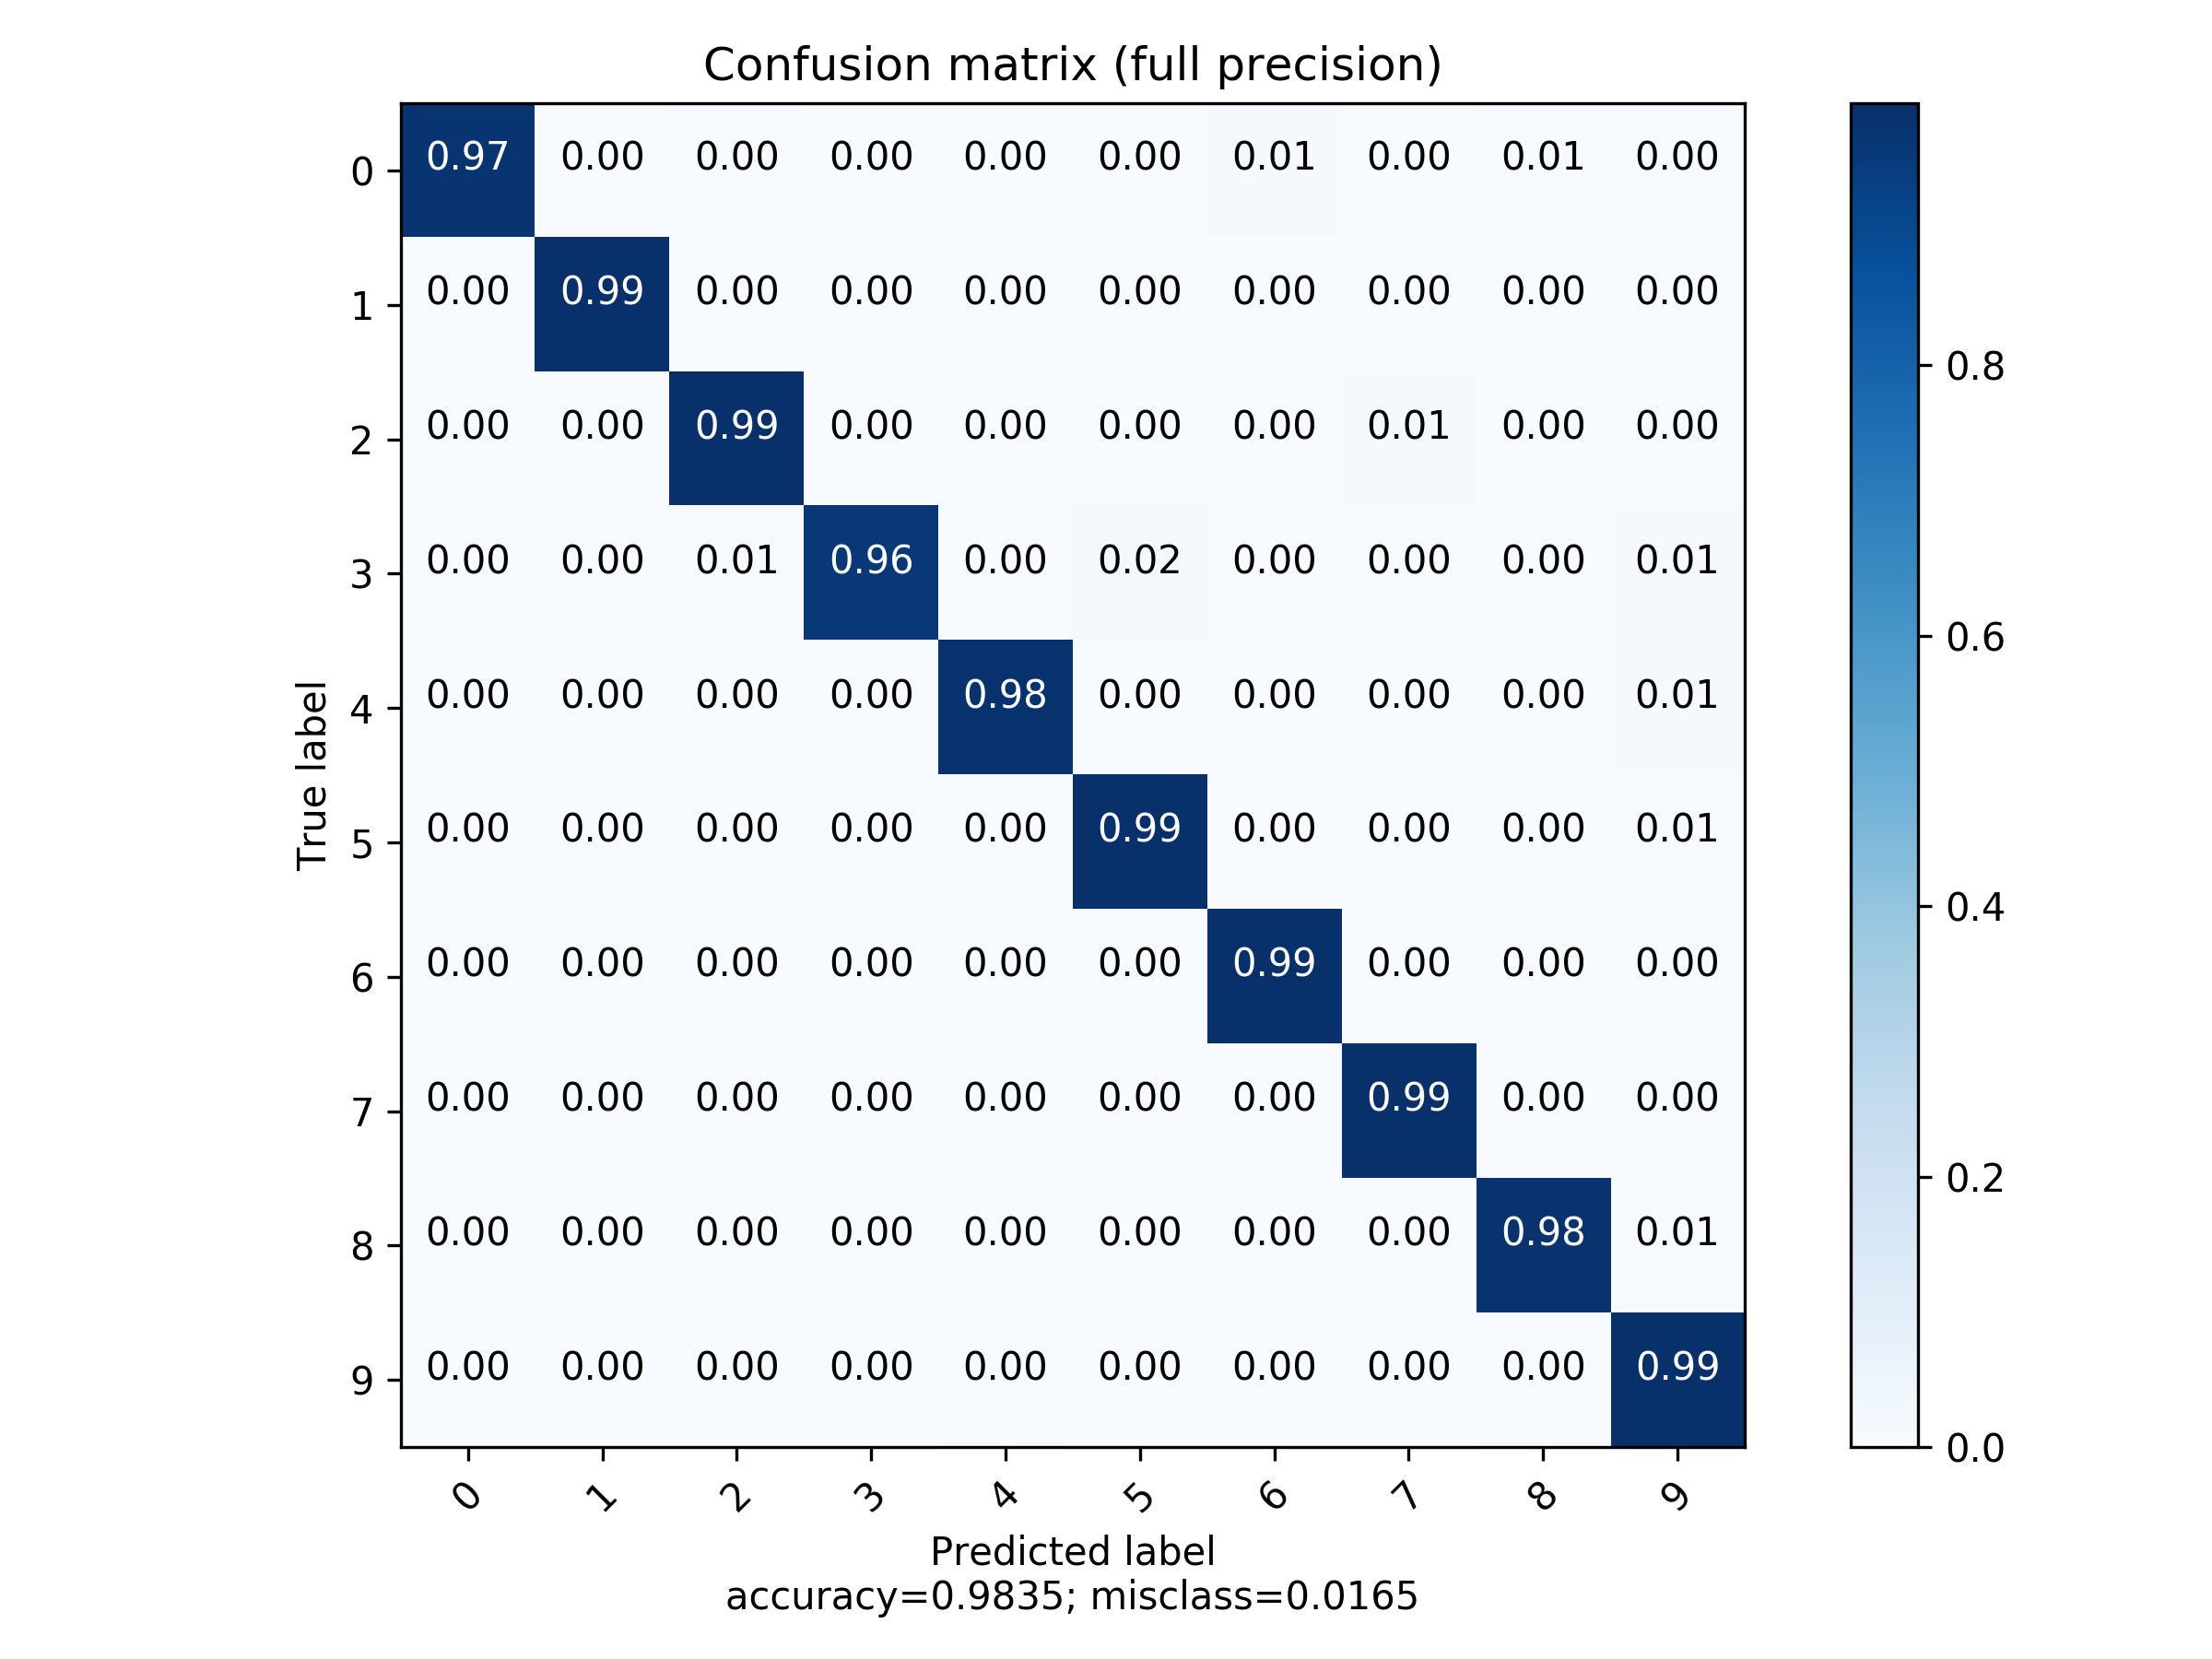
\includegraphics[width=0.9\textwidth]{../../net/images/cm}
	\caption{Floating Point}
	\label{fig:network-test-cm}
\end{subfigure}%
~
\begin{subfigure}[t]{0.5\textwidth}
	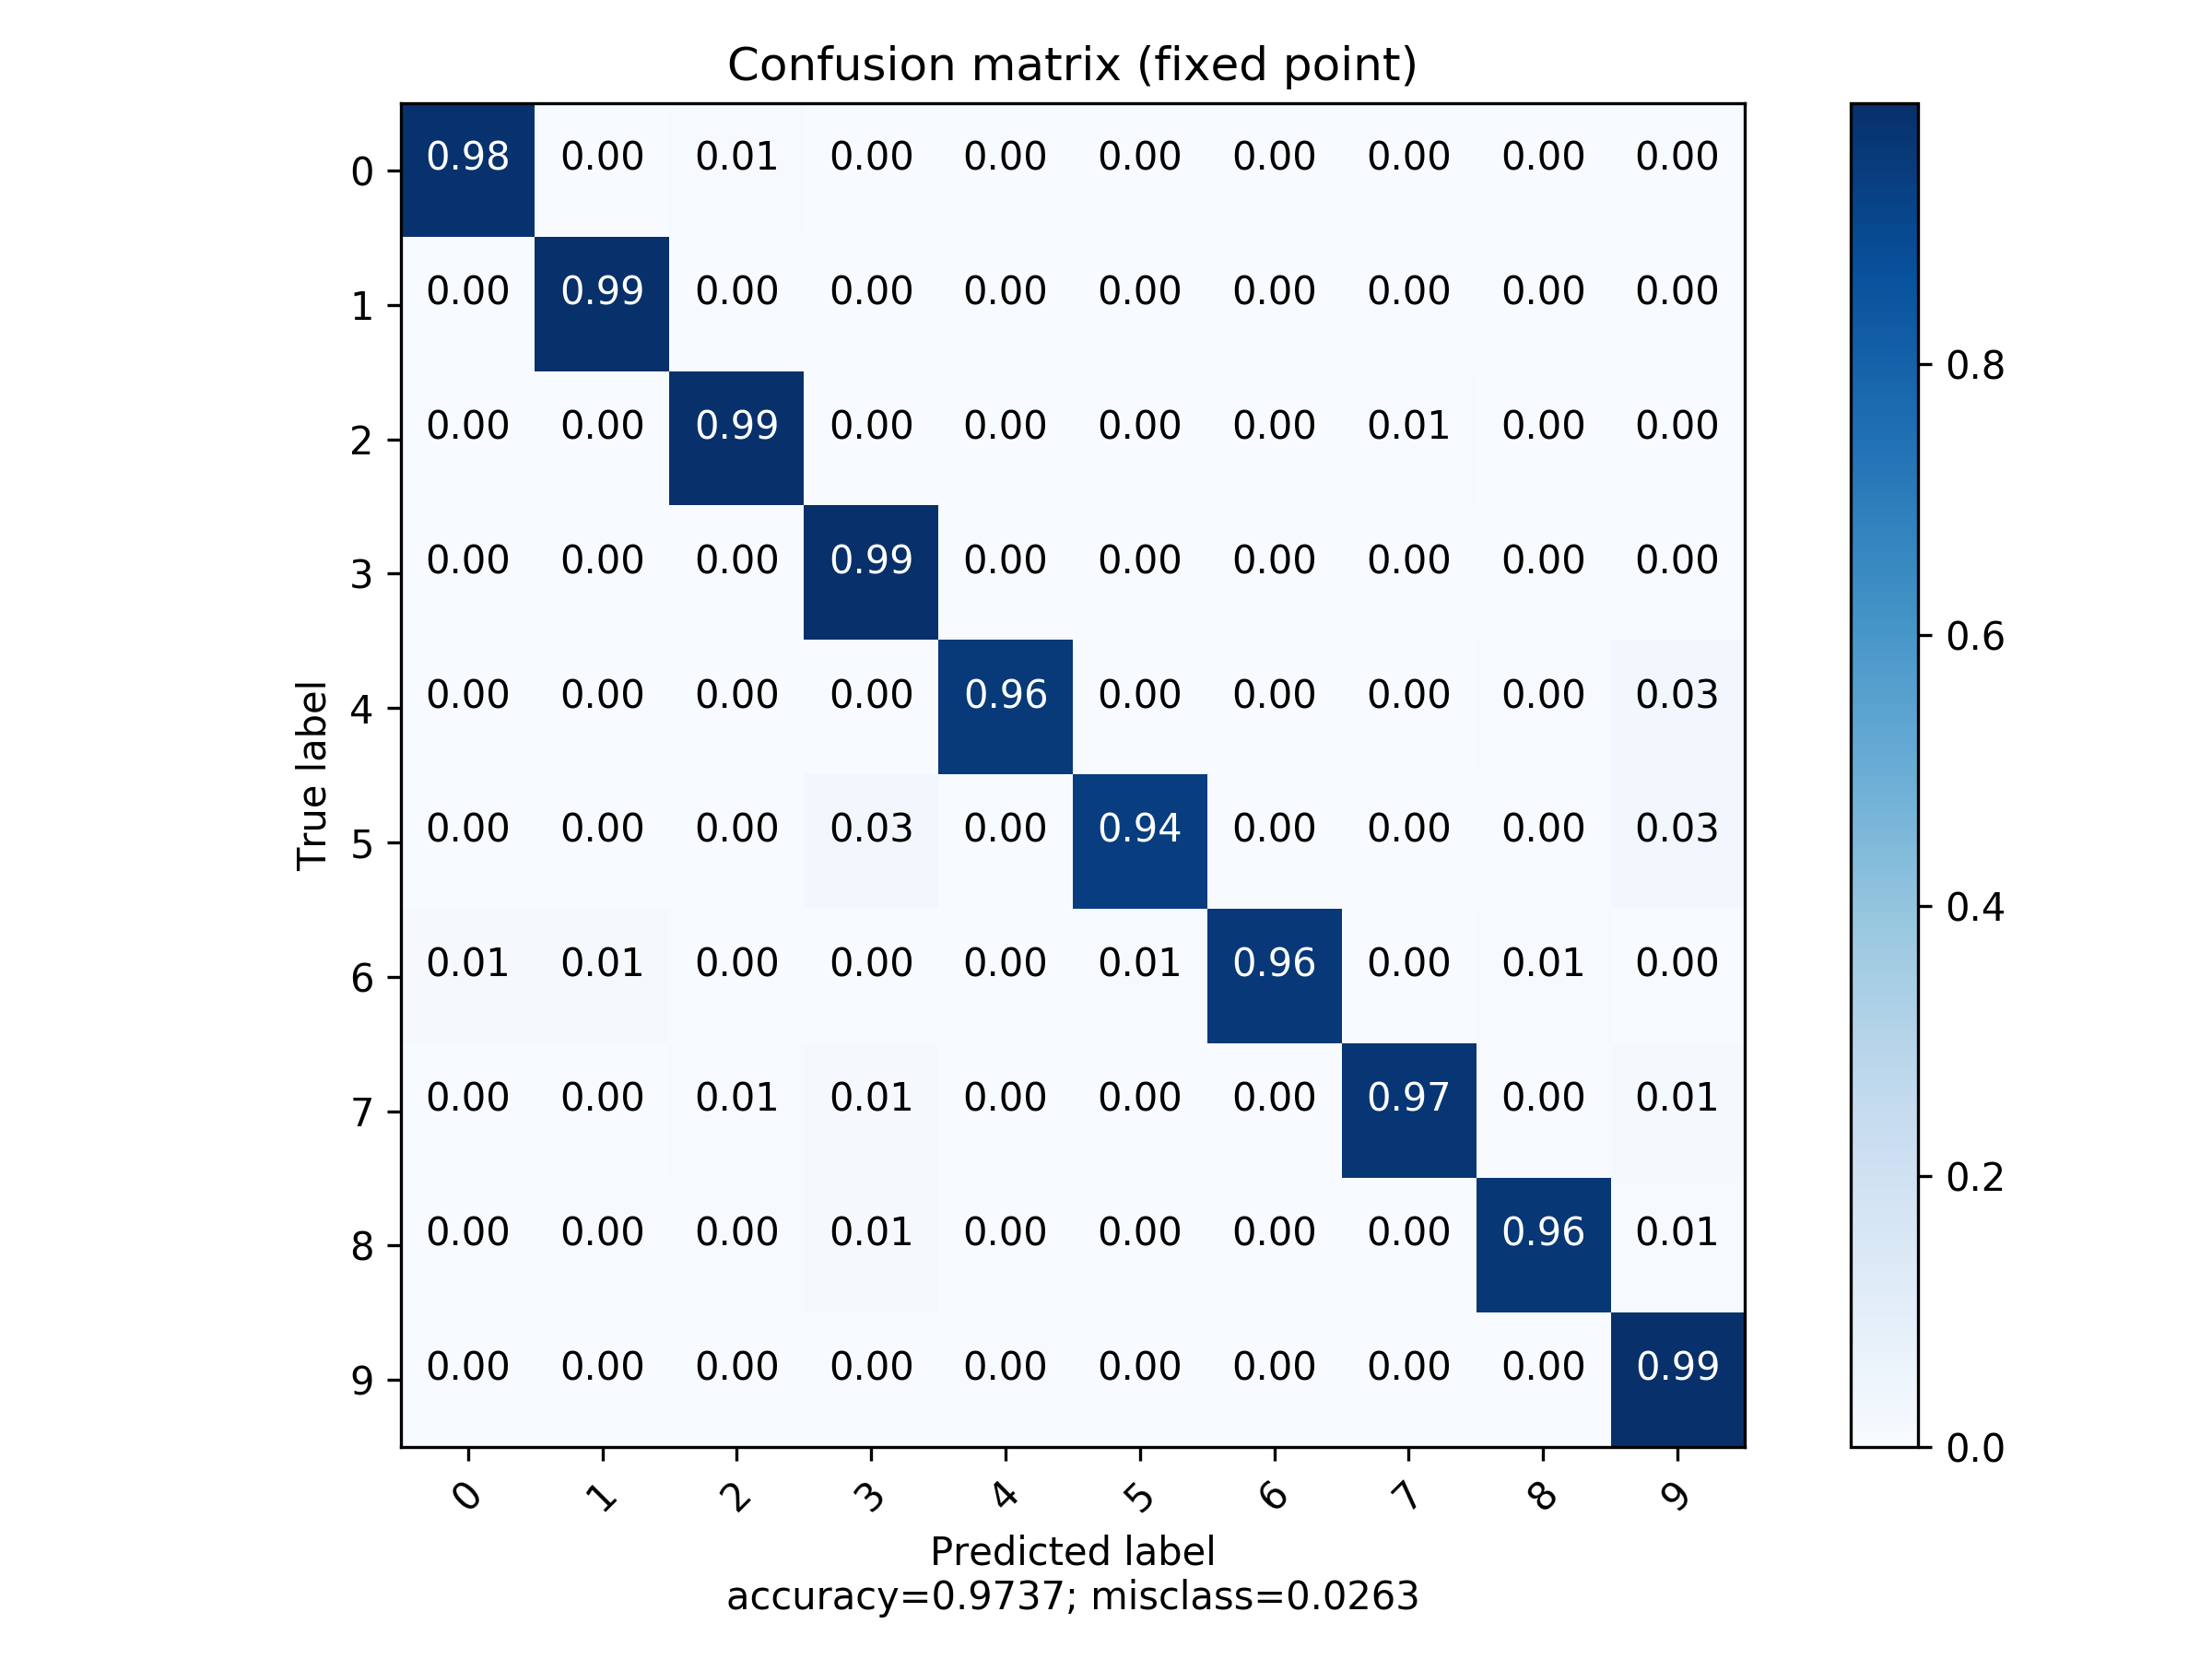
\includegraphics[width=0.9\textwidth]{../../net/images/qcm}
	\caption{Quantized Values}
	\label{fig:network-test-qcm}
\end{subfigure}
\caption{Confusion matrix for the floating point and quantized version of the network.}
\label{fig:network-confusion-matrix}
\end{figure}


\subsection{Quantization}
\label{sec:nn-quant}

The network is trained and created using \SI{32}{\bit} floating point values in Python. Directly porting this all the weights and biases to the FPGA is due to the limited amount of available resources not feasible. The goal is therefore to reduce the amount of required hardware cells by switching from floating point arithmetic to the less expensive integer arithmetic. Then a floating point value $v$ can be approximately represented as 
\begin{equation}
	v \approx Q \cdot 2 ^{-m}
\end{equation}
where $Q$ and $m$ are integers. In our case all input values of the first layer are guaranteed to lie in the interval $[0,1]$ and all layer weights are known from training. It is therefore possible to precompute the expected range where the output values will be. Depending on this range it is then possible to select a suitable bit width for both $Q$ and $m$.

This is a cost-accuracy trade-off where higher bit widths would improve accuracy as well as increase the amount of hardware resources needed.
In \cite{Wu:2018aa} different strategies of choosing bit widths for $Q$ and $m$ are compared and they observed three main configurations, which are (from simple to advanced):
\begin{enumerate}
	\item Use a $(Q,m)$ configuration for the whole network
	\item Use a $(Q,m)$ configuration for each layer
	\item Use a $(Q,m)$ configuration for each output channel 
\end{enumerate}
In the third configuration the authors could reduce the bit widths the most without sacrificing accuracy this increases the complexity in transferring the weights from layer to layer because the additional shift operations are necessary in order to adjust for the different values of $m$.
In \cite{Wu:2018aa} the authors also deduced from their experiments that the accuracy of the weights can be reduced the most, followed by the activations. By analysing the weights of our network (see Figure~\ref{fig:network-weight-distributions}) a per channel quantization is not necessary, because all weights in a Convolutional Layer are equally distributed among the output channels. Another important property that can be noted is the that the weights do have zero mean and most of the values lie very close to zero. Because of the usage of ReLU layer the situation is different for the activations where unsigned integers can be used, the distributions are shown in Figure~\ref{fig:network-activations-distributions}.

Using the distribution histograms we then derived the necessary bitwidths for $Q$ and $m$. In our experiments we were able to reduce them to \SI{8}{\bit}, if we used a single configuration for the whole network and also reducing them down to \SI{4}{\bit} if the bitwidth configuration is selected for each layer independently with an accuracy drop from around \SI{98.35}{\percent} to \SI{97.37}{\percent}. The strategy to the select the values for $(Q,m)$ was
\begin{enumerate}
	\item Find the value range of the weights and output activations of each layer
	\item Select suitable $(Q,m)$ values that most activations fall in that range
	\item Calculate the bit widths and exponents of the multiplication operation
	\item Add $\lceil \log_2(n) \rceil$ extra bits to account for the accumulation of $n$ values
	\item Compare the accumulated exponents and with the exponents of the successive layers input exponents. The difference is the amount of shift required
\end{enumerate}
It is noteworthy that the values for $m$ do not need to be stored in the final network, because those are only used to determine the amount of shifts between the layers. Also the values need to be clipped to their maximum and minimum values. The complete configuration of the network is summarized in Table~\ref{tab:quantization-linear-params}.

Ad 4 and 5: The transition from a layer to the next often changes the exponent $m$ and the available bitwidth. To account for this the values need to accordingly shifted. Also the decreased bitwidth needs clipping to maximum available values for the target bitwidth. This directly alters the behaviour of the network which should be accounted for during training, which is done via a saturated version of ReLU, defined as:
\begin{equation}
    \text{ReLU}_{\text{sat}}: ~ f(x;p) = \begin{cases}
		0 	\quad \text{if} \quad x < 0 \\
		p 	\quad \text{if} \quad x > p \\
		x	\quad \text{else}
	\end{cases}
\end{equation}

For our network only linear quantization has been used but also non-linear quantization, e.g. in a $\log_2$ way which is proposed in \cite{Lee:2017aa}. Experiments showed that using this technique even further down to \SI{3}{\bit} weights in our case.
Another optimization technique that could be explored is the systematically removing of weights (connections) of the network and reduce the amount of operations needed to be performed, a process referred to as ''pruning'' \cite{Zhu:2017aa}. This was not explicitly performed but is implicitly done by low bit quantization.

\begin{table}[hbt]
  \centering
  \begin{tabular}{lcccc}
	\toprule
    Network Part 	  & $|Q|$ & $m$ & $\pm$ & $v$ (real value range) \\
	\midrule
    Input 		 	  &  8    & 8  & $+$   & $[0,1]  $ \\
    L1: Weights 	  &  4    & 2  & $\pm$ & $[-2,2] $ \\
    L1: Intermediates & 12    & 10 & $\pm$ & $[-2,2] $ \\
    L1: Accumulated   & 16    & 10 & $\pm$ & 		   \\
    \midrule
    L1 $\to$ L2 	  & \multicolumn{4}{c}{Rshift by $10-2$ and clip values in range $[0,15]$} \\
    \midrule
    L2: Input 		  &  4    & 2  & $+$   & $[-2,2] $ 	   \\
    L2: Weights 	  &  4    & 5  & $\pm$ & $[-0.5,0.5] $ \\
    L2: Intermediates &  8    & 7  & $\pm$ & $[-1,1] $ \\
    L2: Accumulated   & 16    & 7  & $\pm$ &  			   \\
    \midrule
    L2 $\to$ L3 	  & \multicolumn{4}{c}{Rshift by $7-0$ and clip values in range $[0,15]$} \\
    \midrule
    L3: Input 		  &  4    & 0  & $+$   & $[0,15] $     \\
    L3: Weights 	  &  4    & 5  & $\pm$ & $[-0.5,0.5] $ \\
    L3: Intermediates &  8    & 5  & $\pm$ & $[-7.5,7.5] $ \\
    L3: Accumulated   & 19    & 5  & $\pm$ &               \\
    \midrule
    L3 $\to$ L4 	  & \multicolumn{4}{c}{Rshift by $5-0$ and clip values in range $[0,15]$} \\
    \midrule
    L4: Input 		  &  4    & 0  & $+$   & $[0,15] $ \\
    L4: Weights 	  &  4    & 5  & $\pm$ & $[-0.5,0.5] $ \\
    L4: Intermediates &  8    & 5  & $\pm$ & $[-7.5,7.5] $ \\
    L4: Accumulated   & 14    & 5  & $\pm$ & $[0,1] $ \\
    \bottomrule
  \end{tabular}
  \caption[Quantization parameters for the \SI{4}{\bit} network]{Quantization parameters for the \SI{4}{\bit} network. The intermediate terms are the values after the multiplication operation and the accumulated term denotes values after summing up of weighted inputs including bias in a channel.}
  \label{tab:quantization-linear-params}
\end{table}


%% WEIGHT DISTTRIBUTIONS
\begin{figure}[htbp]
    \centering
    \begin{subfigure}[t]{0.5\textwidth}
        \centering
        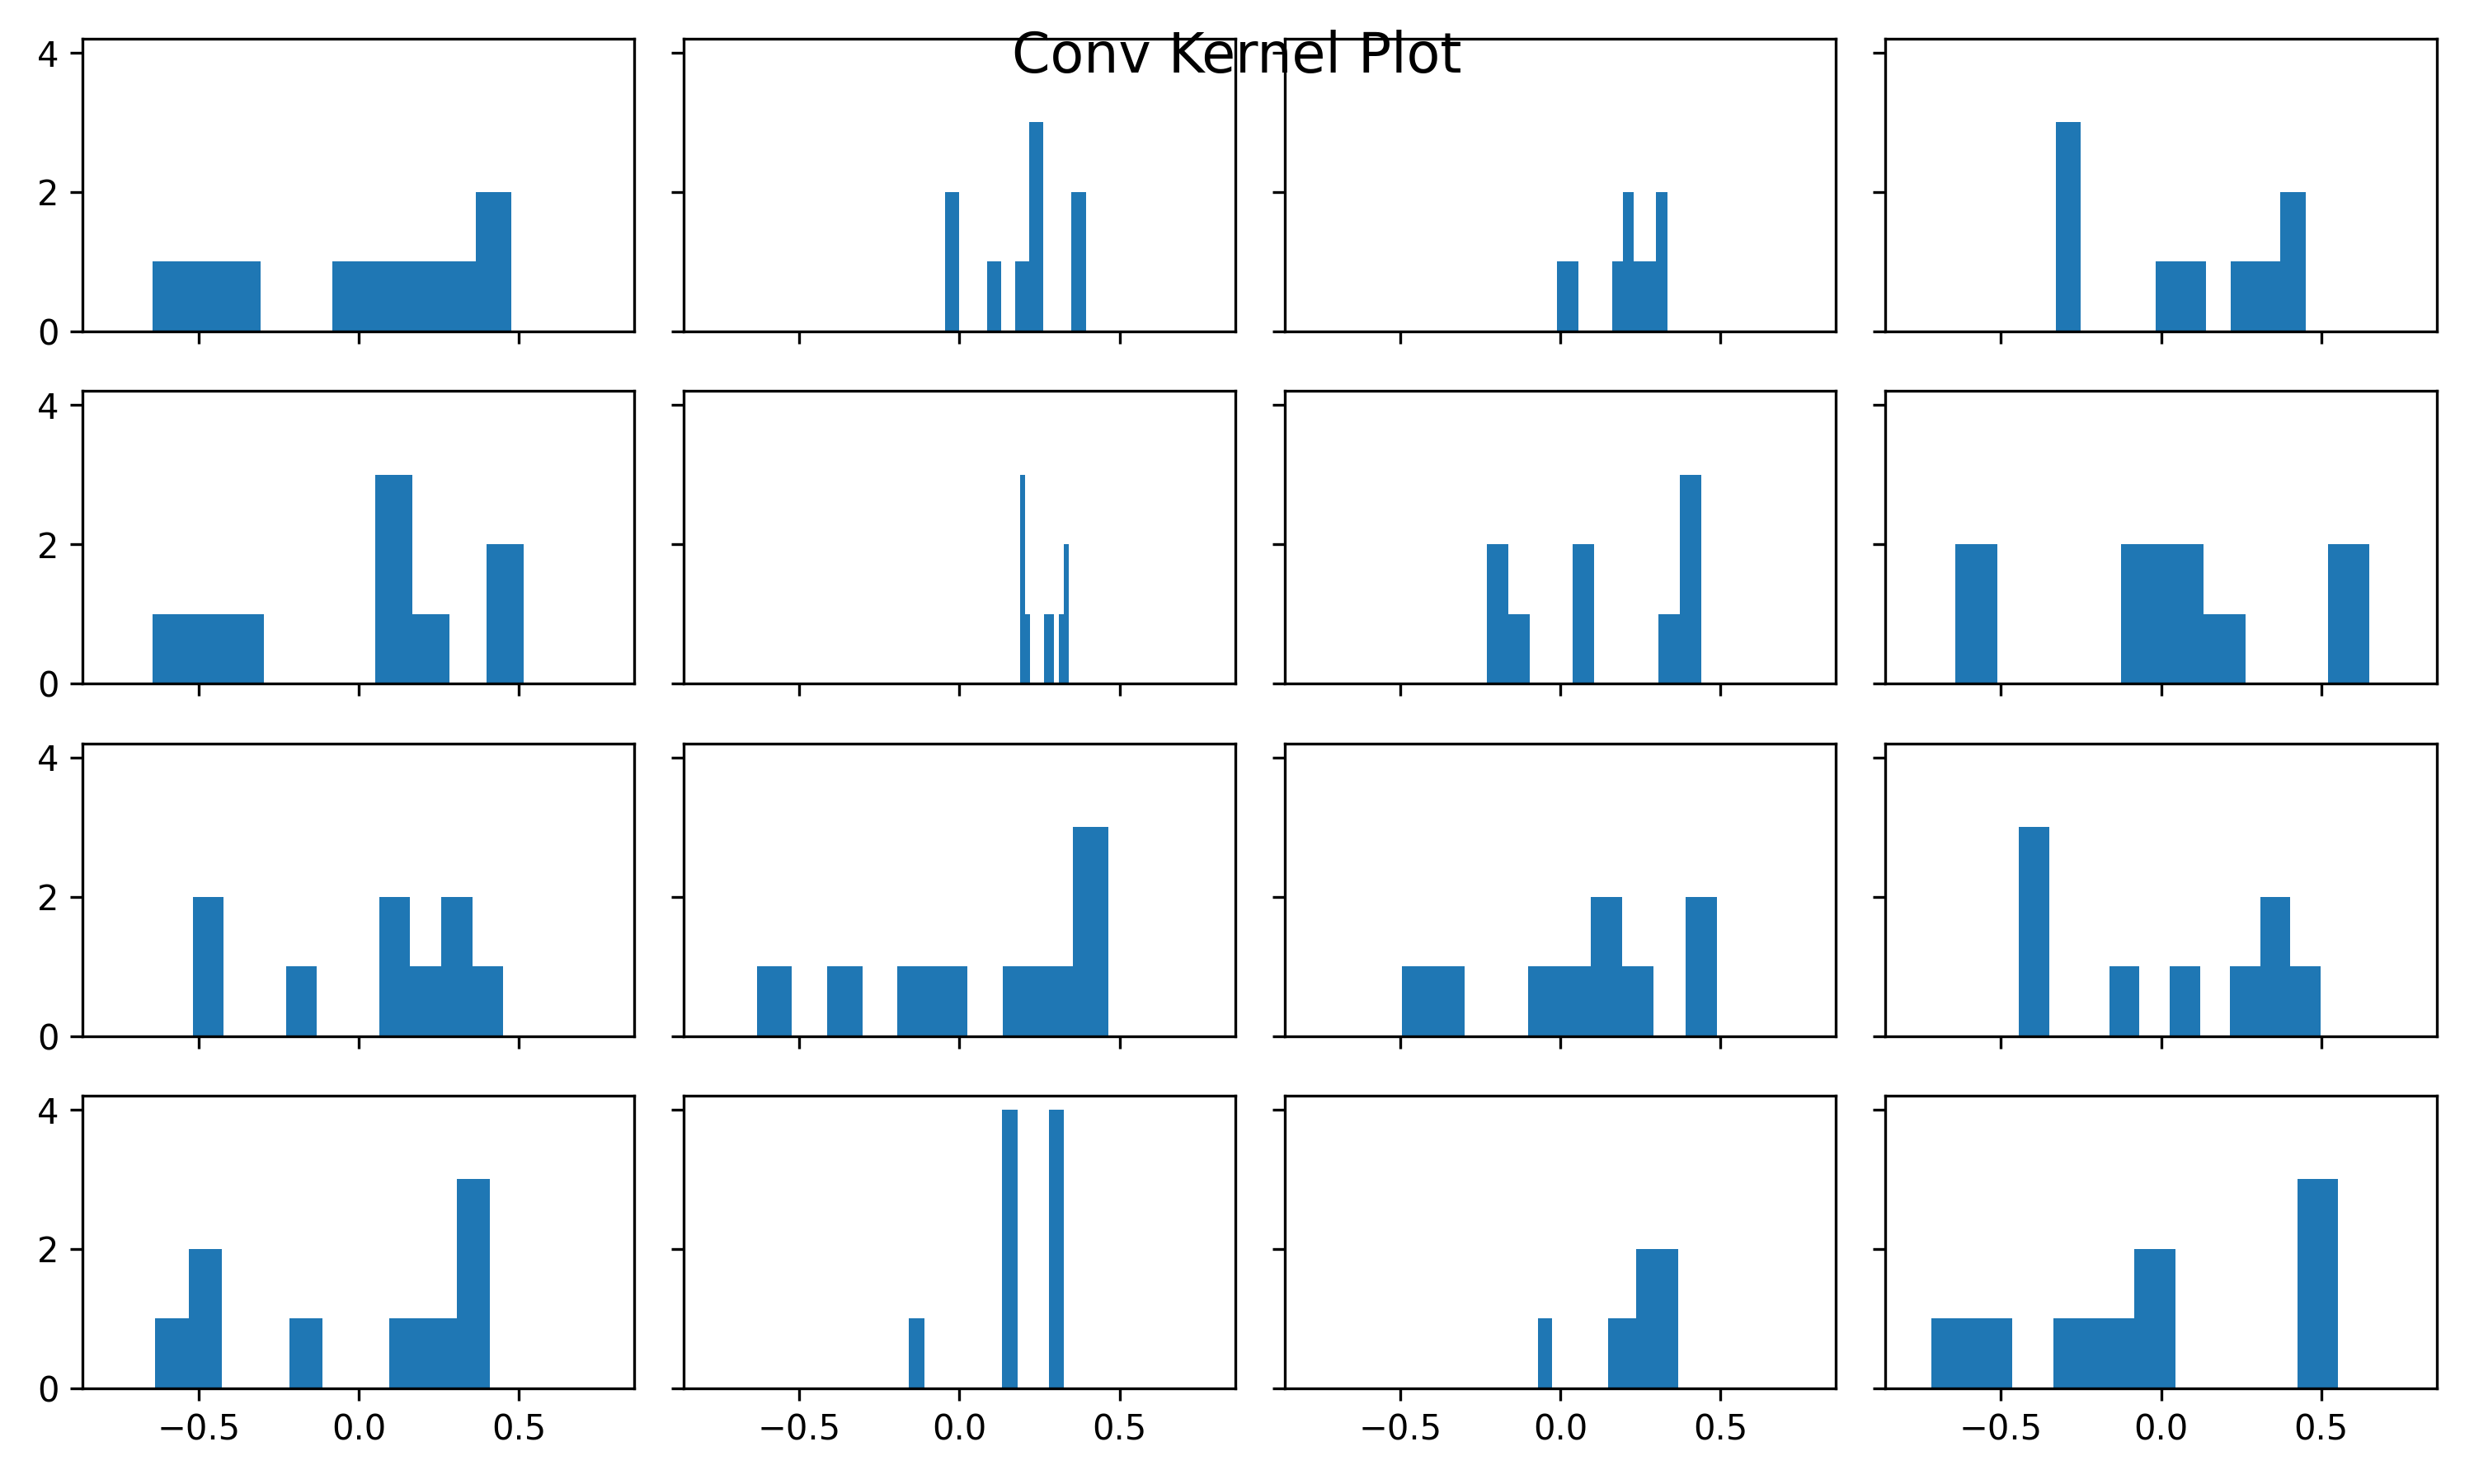
\includegraphics[height=1.6in]{../../net/images/hist_cn1_k}
        \caption{Convolutional Layer 1}
    \end{subfigure}%
    ~ 
    \begin{subfigure}[t]{0.5\textwidth}
        \centering
         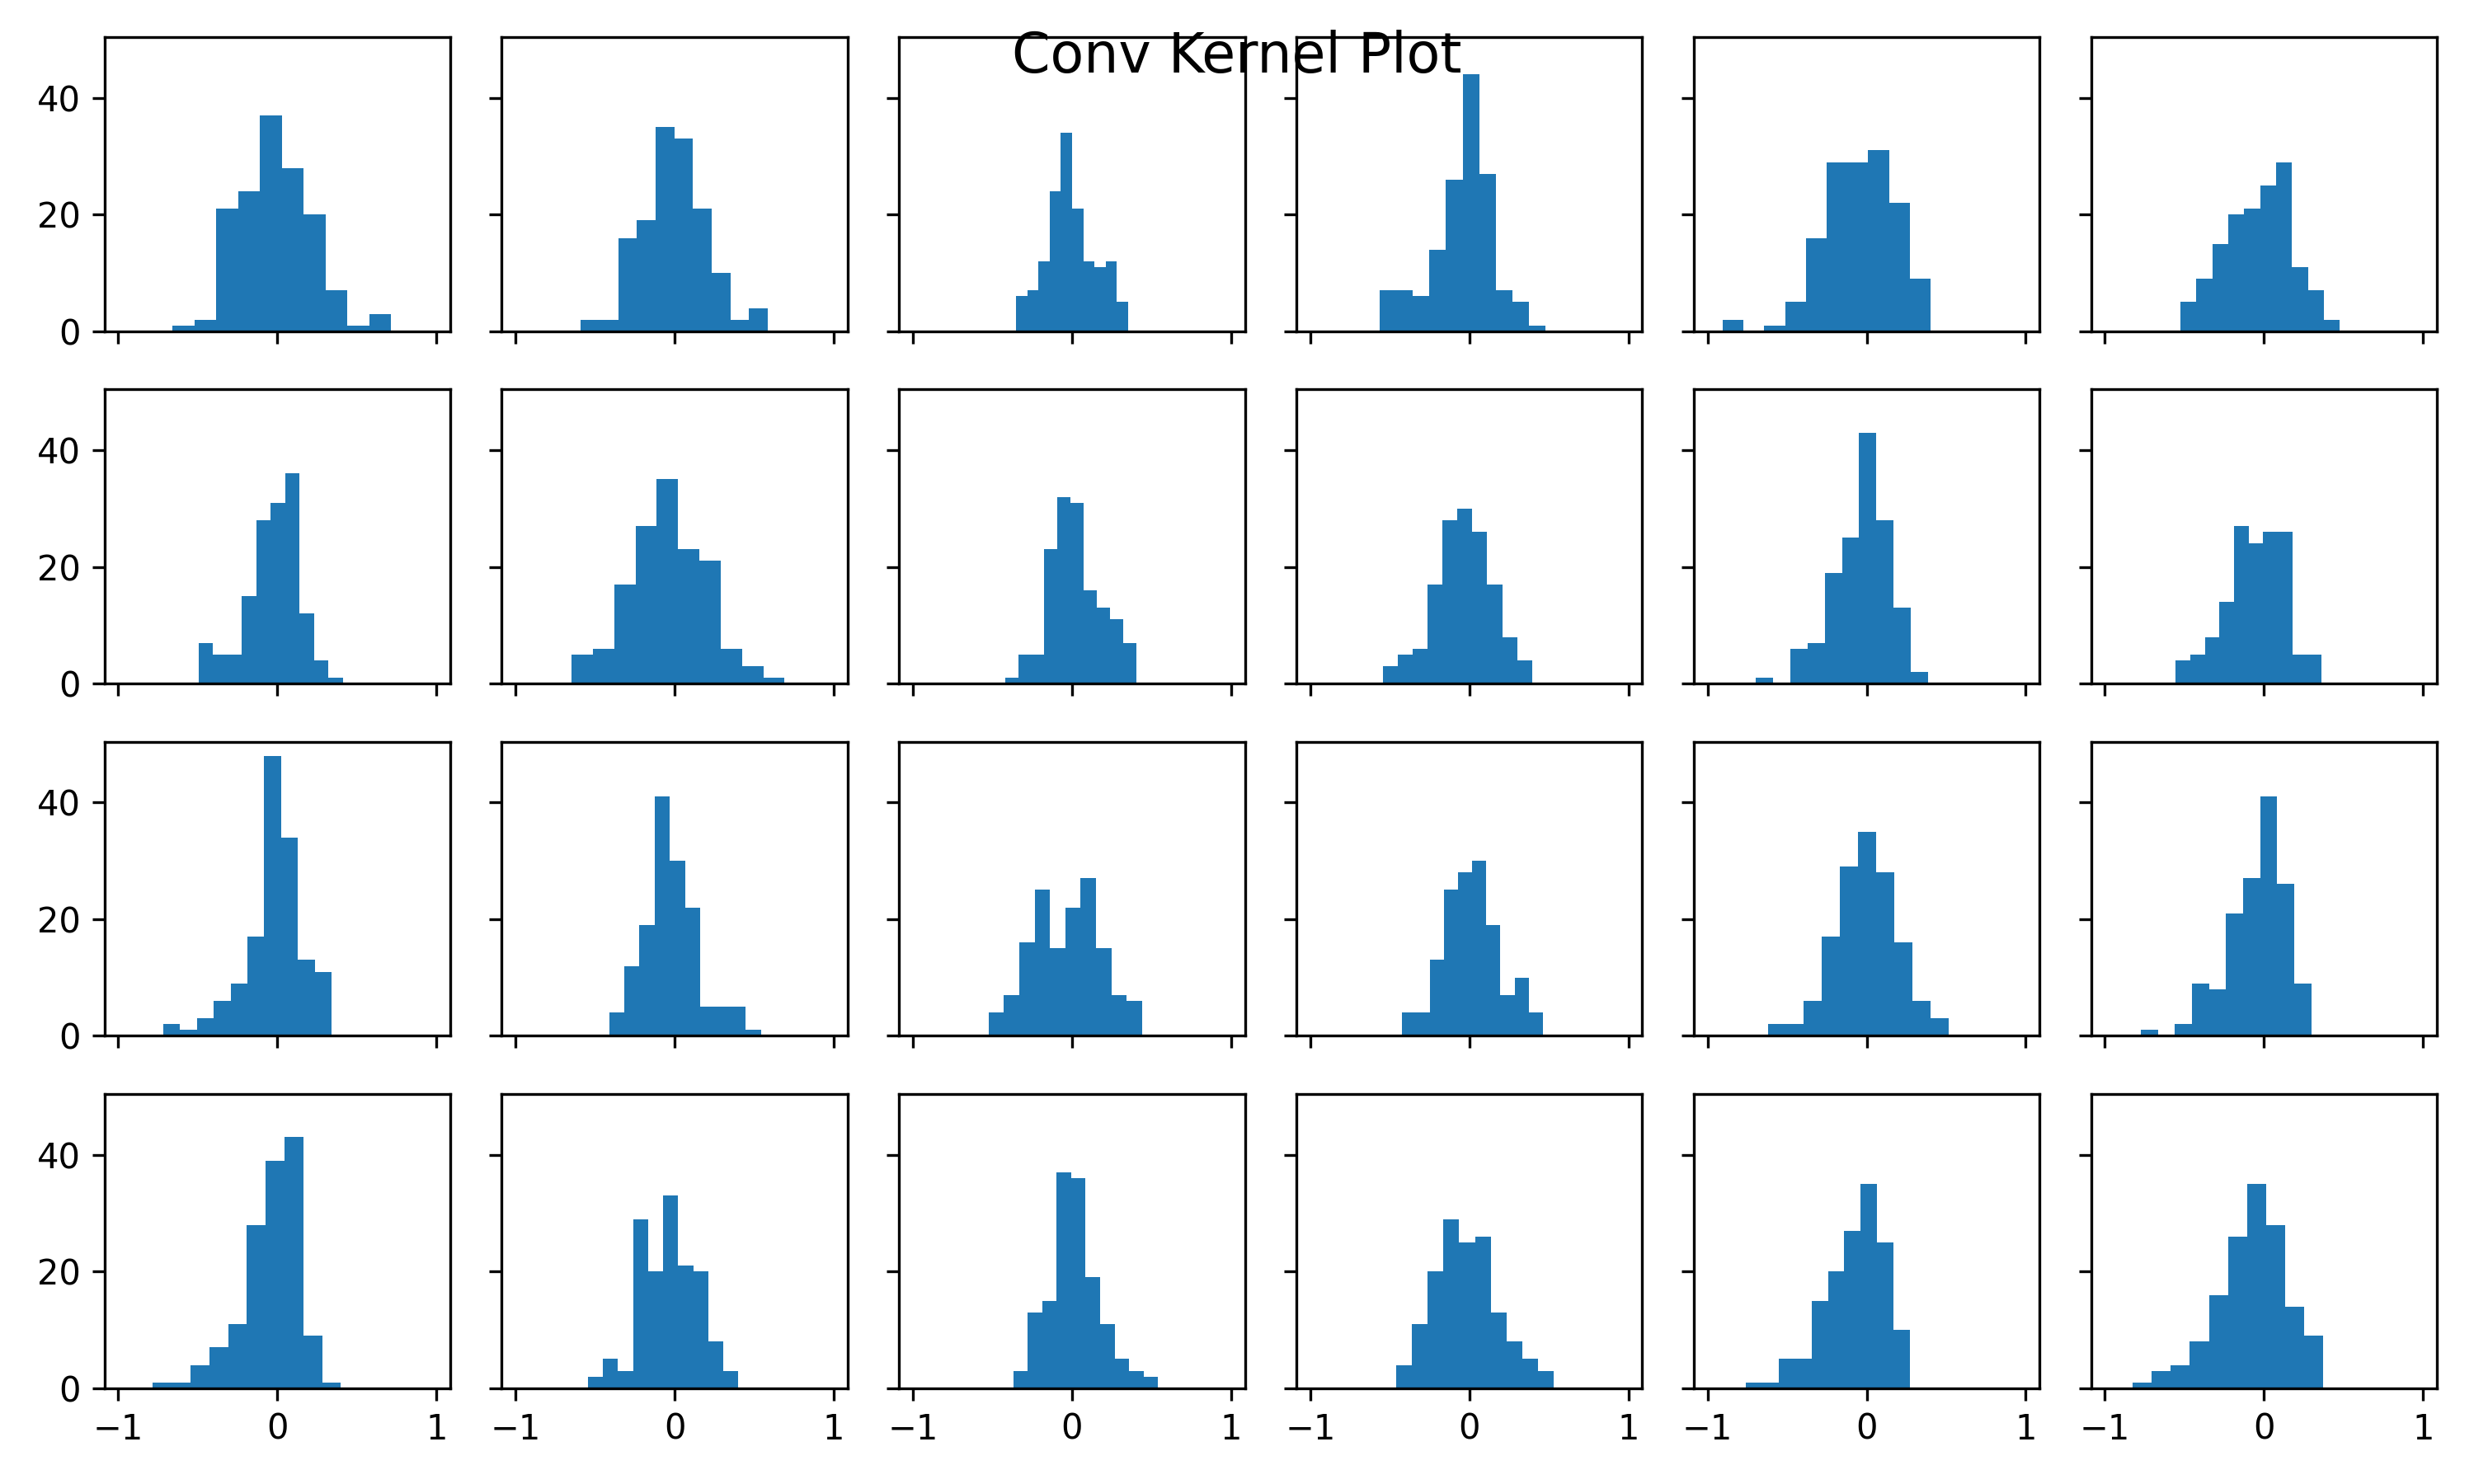
\includegraphics[height=1.6in]{../../net/images/hist_cn2_k}
        \caption{Convolutional Layer 2}
    \end{subfigure}%
    \\
    \begin{subfigure}[t]{0.5\textwidth}
        \centering
        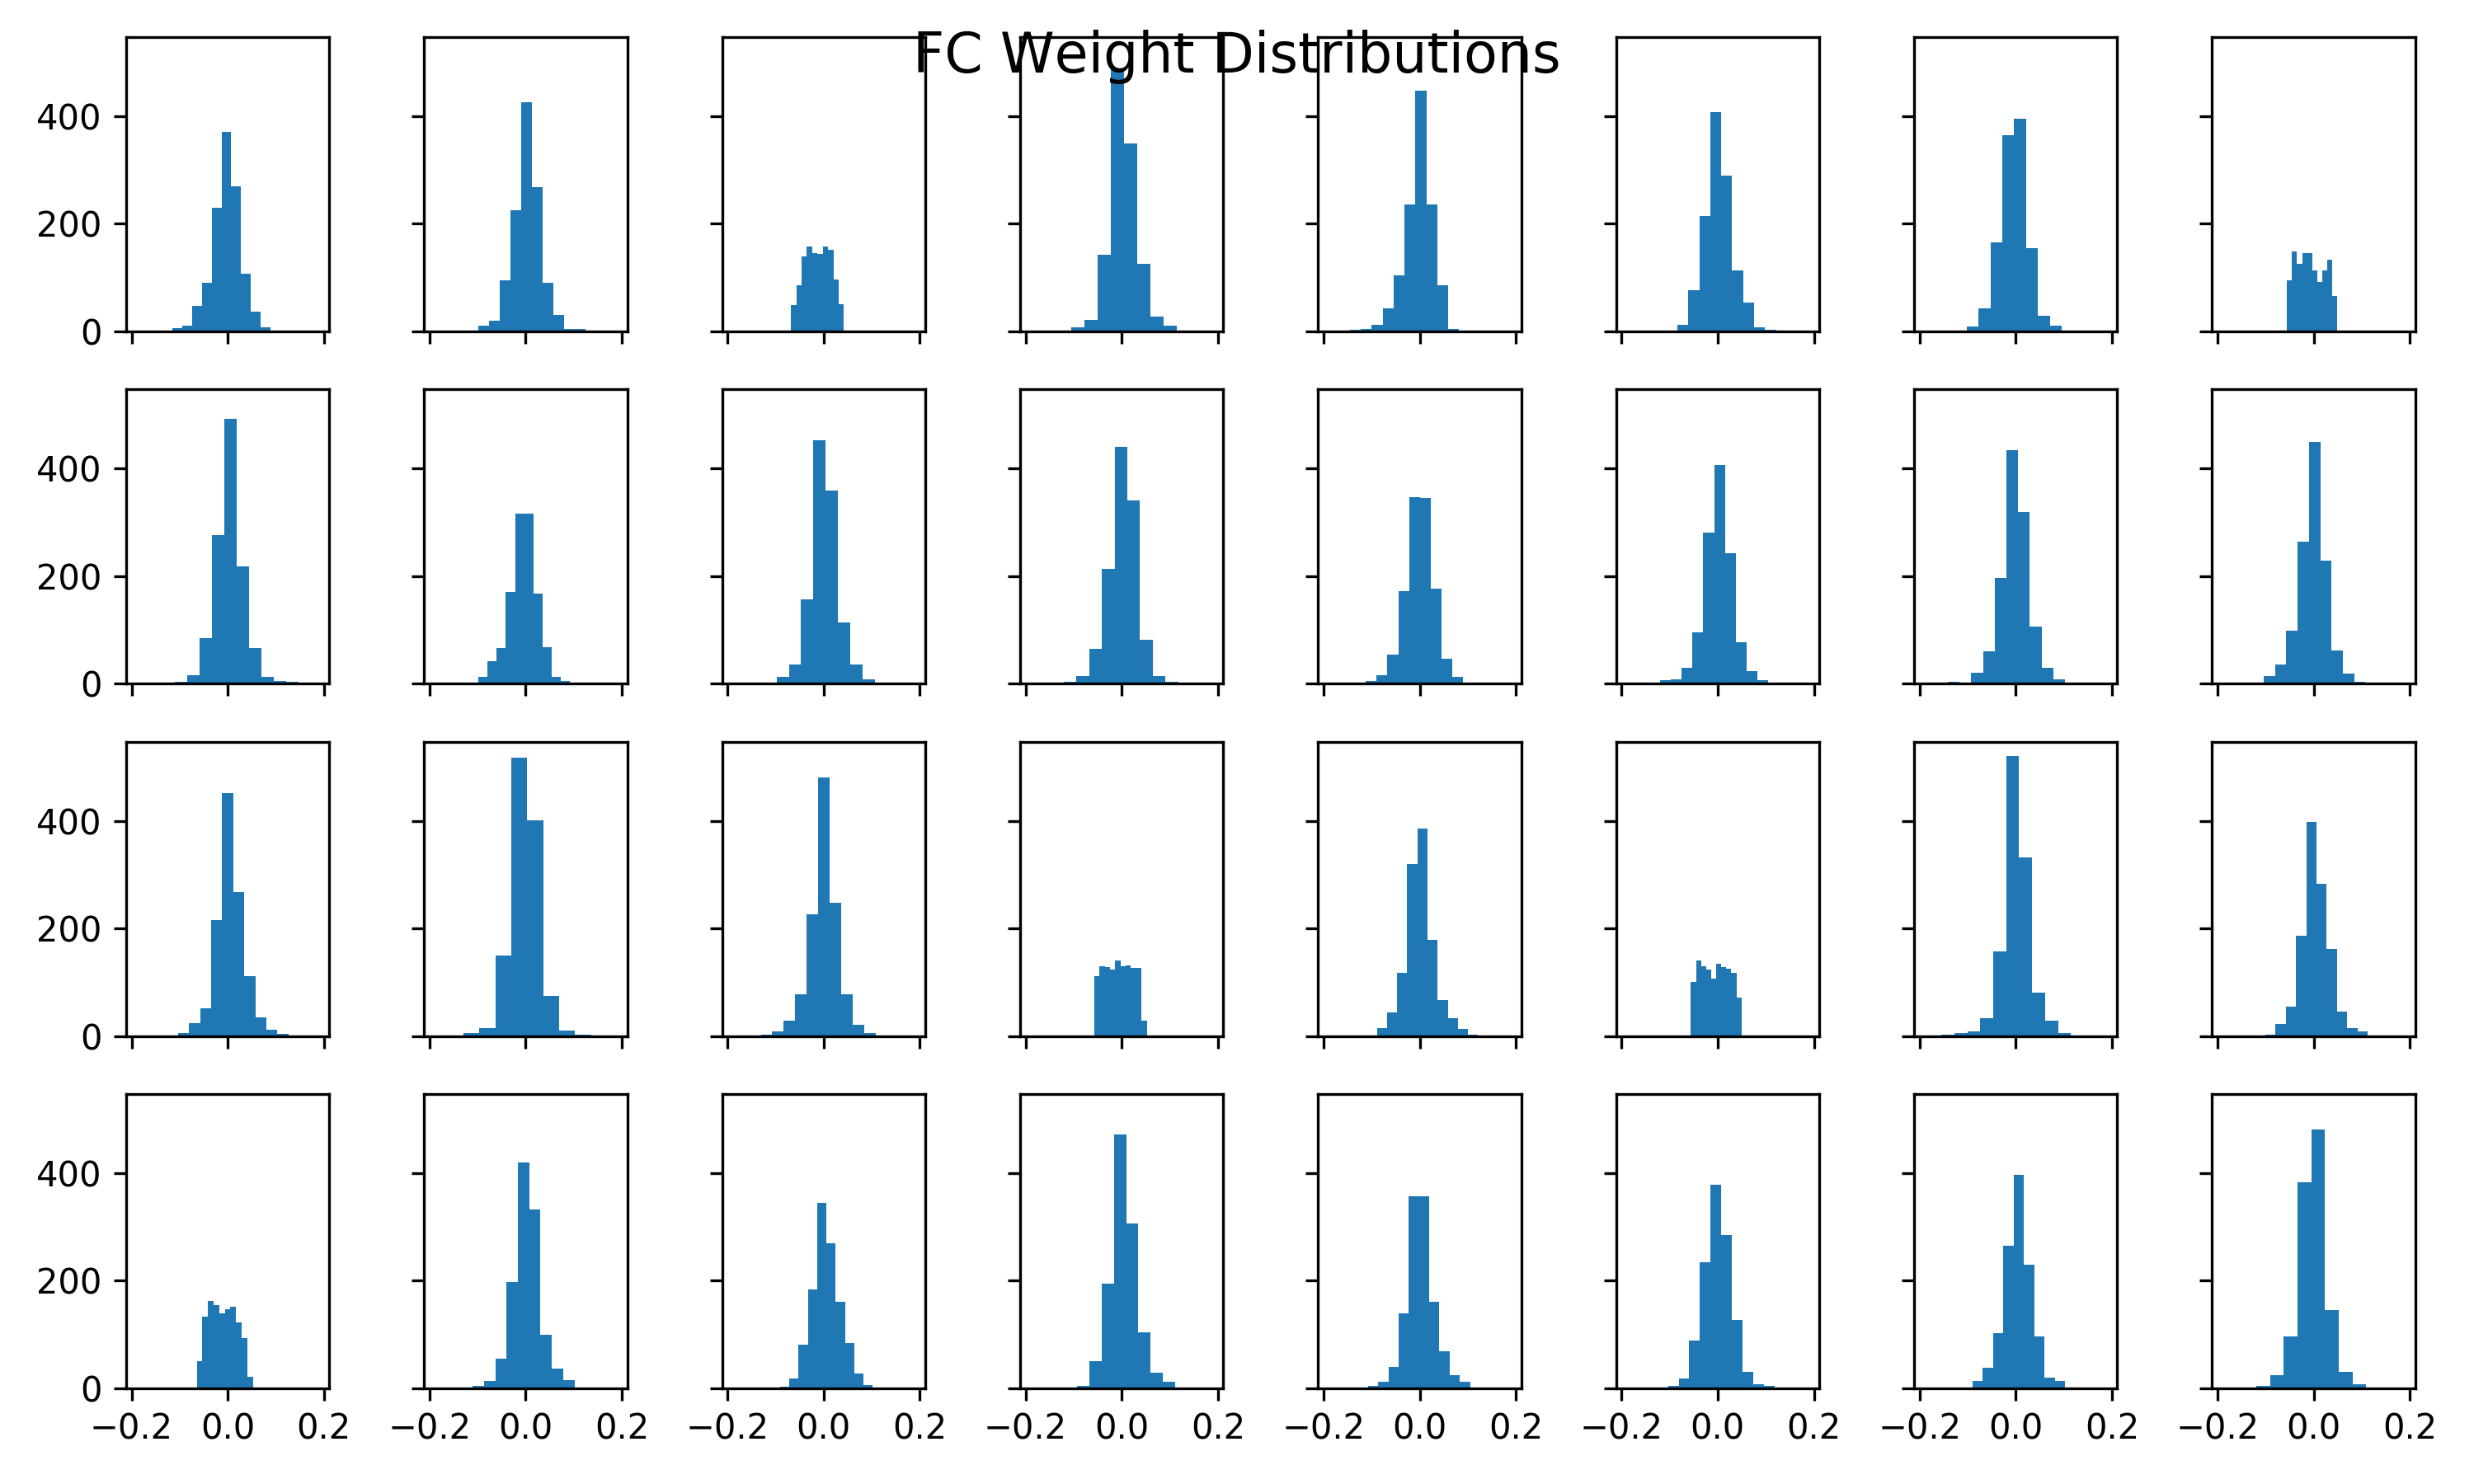
\includegraphics[height=1.6in]{../../net/images/hist_fc1_w}
        \caption{Fully Connected Layer 1}
    \end{subfigure}%
    ~ 
    \begin{subfigure}[t]{0.5\textwidth}
        \centering
         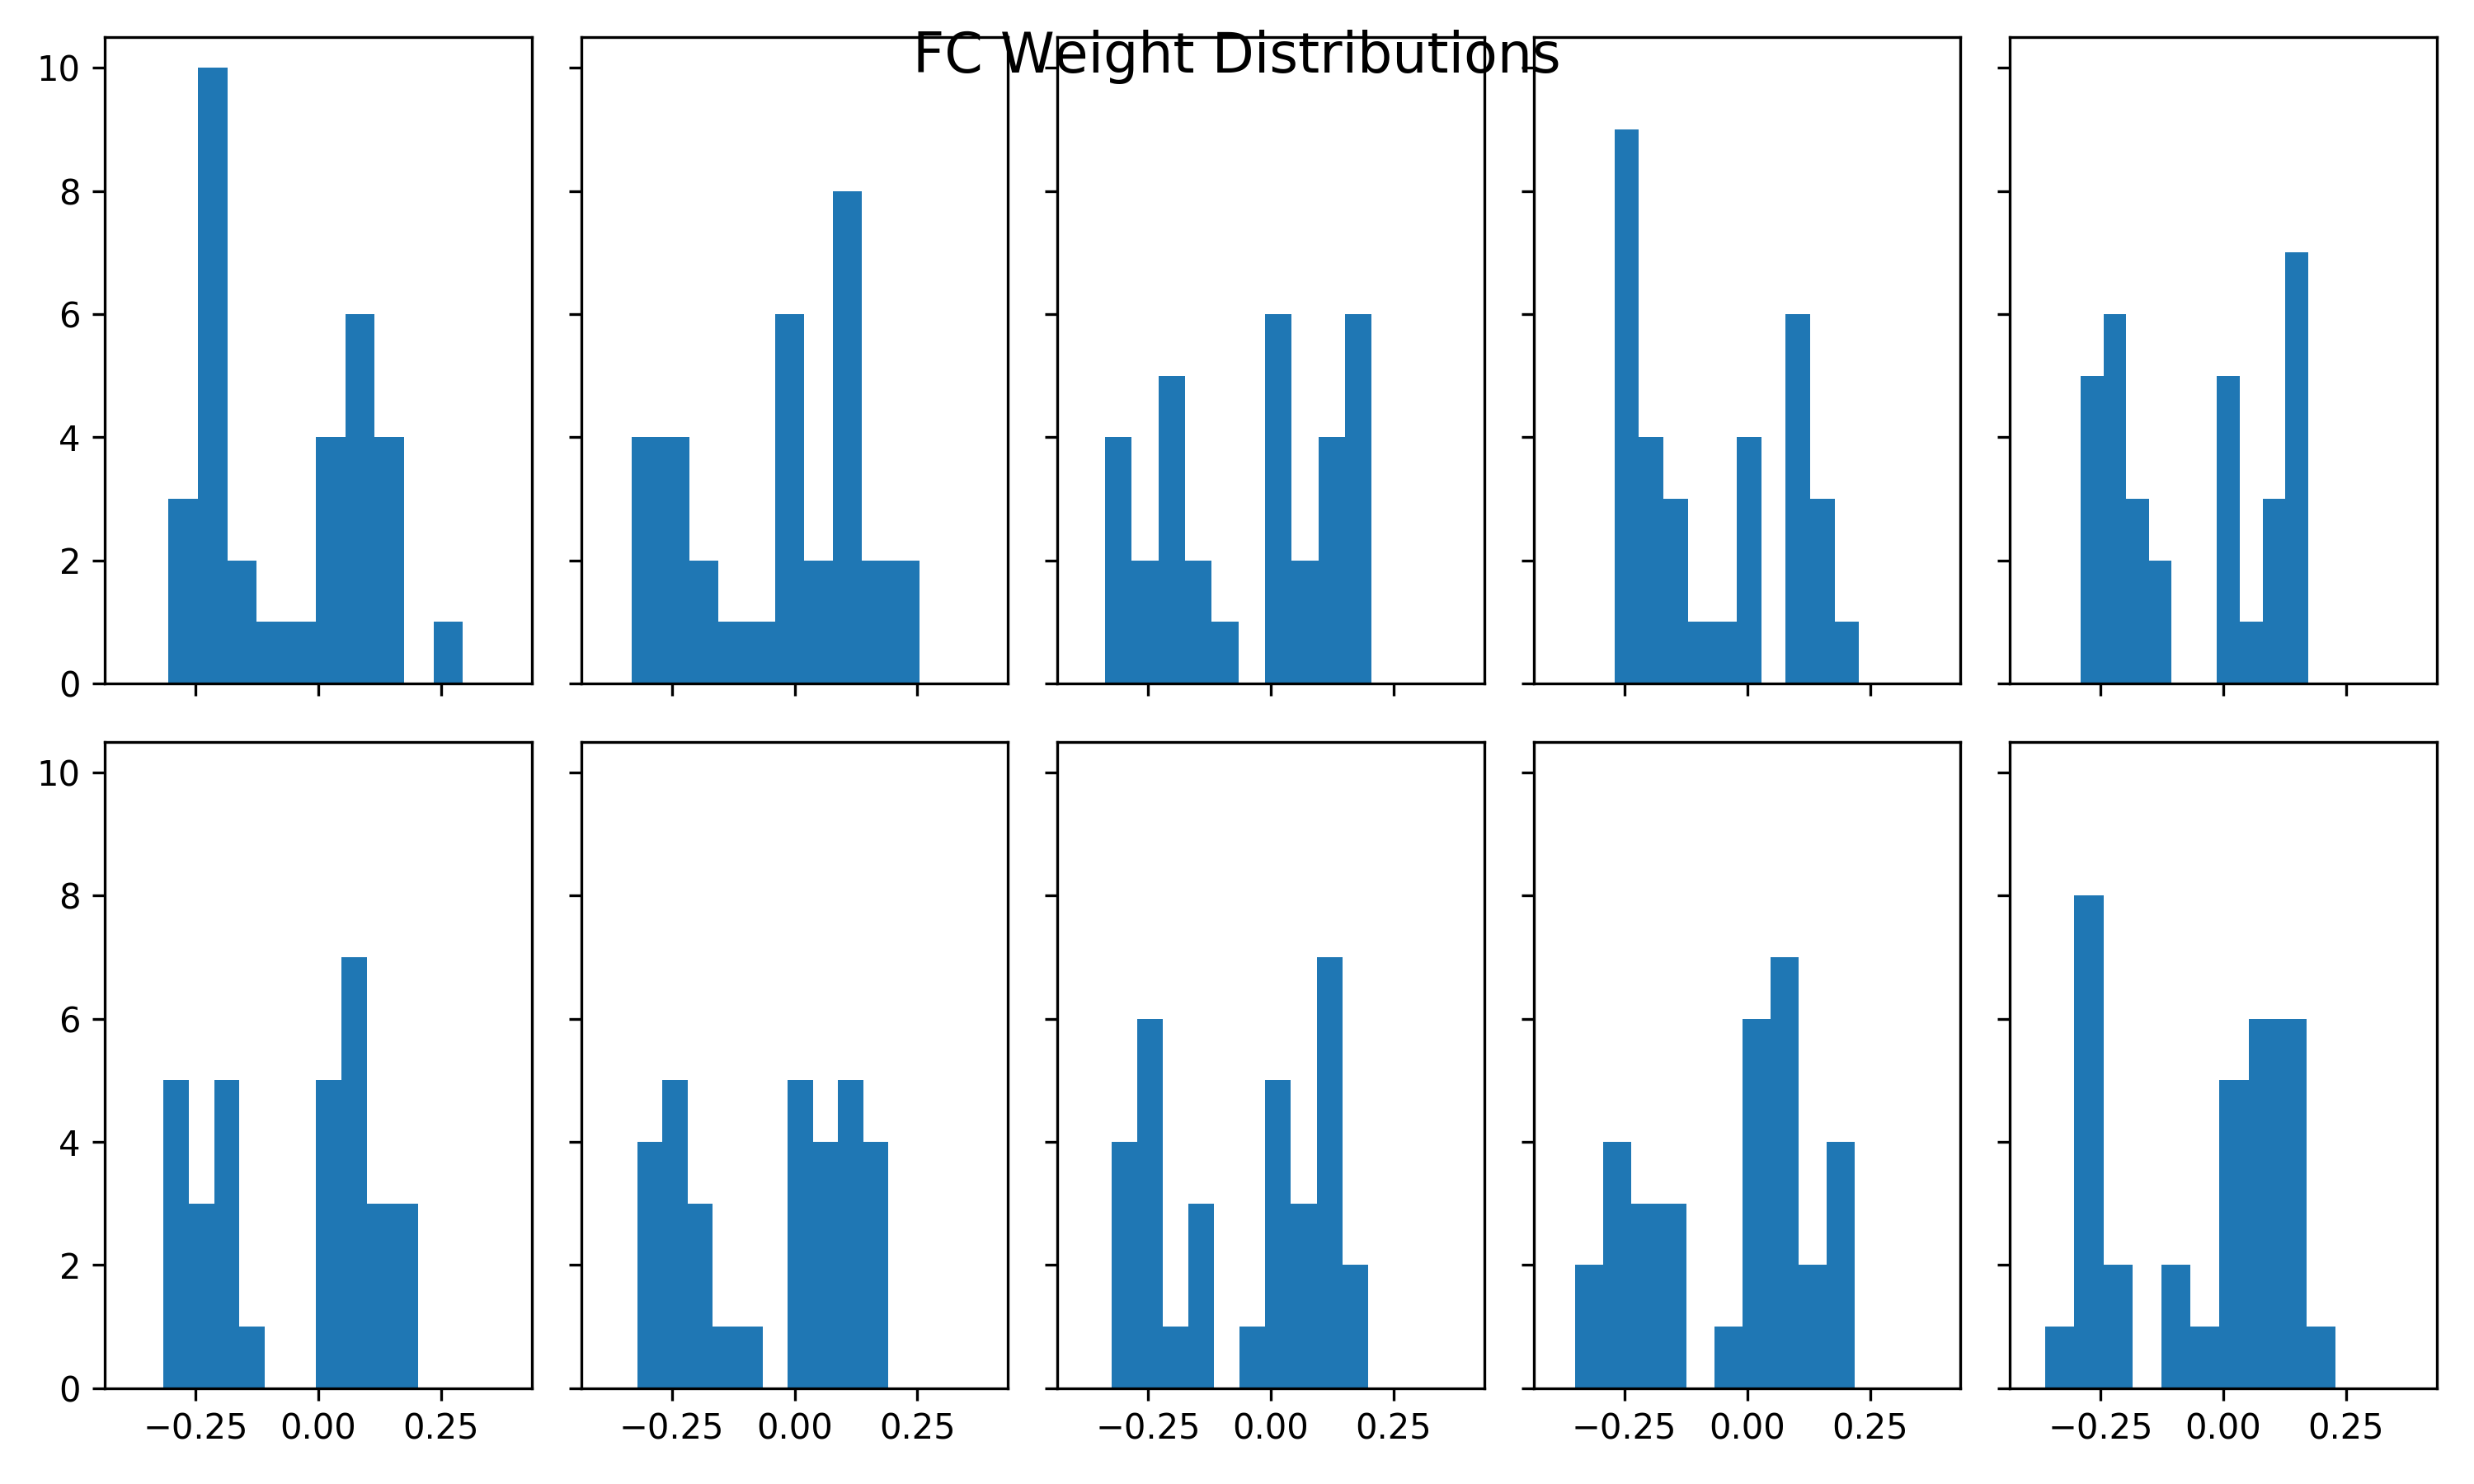
\includegraphics[height=1.6in]{../../net/images/hist_fc2_w}
        \caption{Fully Connected Layer 2}
    \end{subfigure}
    \caption[Distribution of the network weights for the different layers]{Distribution of the network weights for the different layers. It can be seen that the weights are distributed close to zero.}
    \label{fig:network-weight-distributions}
\end{figure}


%% ACTIVATIONS DISTTRIBUTIONS
\begin{figure}[htbp]
    \centering
    \begin{subfigure}[t]{0.5\textwidth}
        \centering
        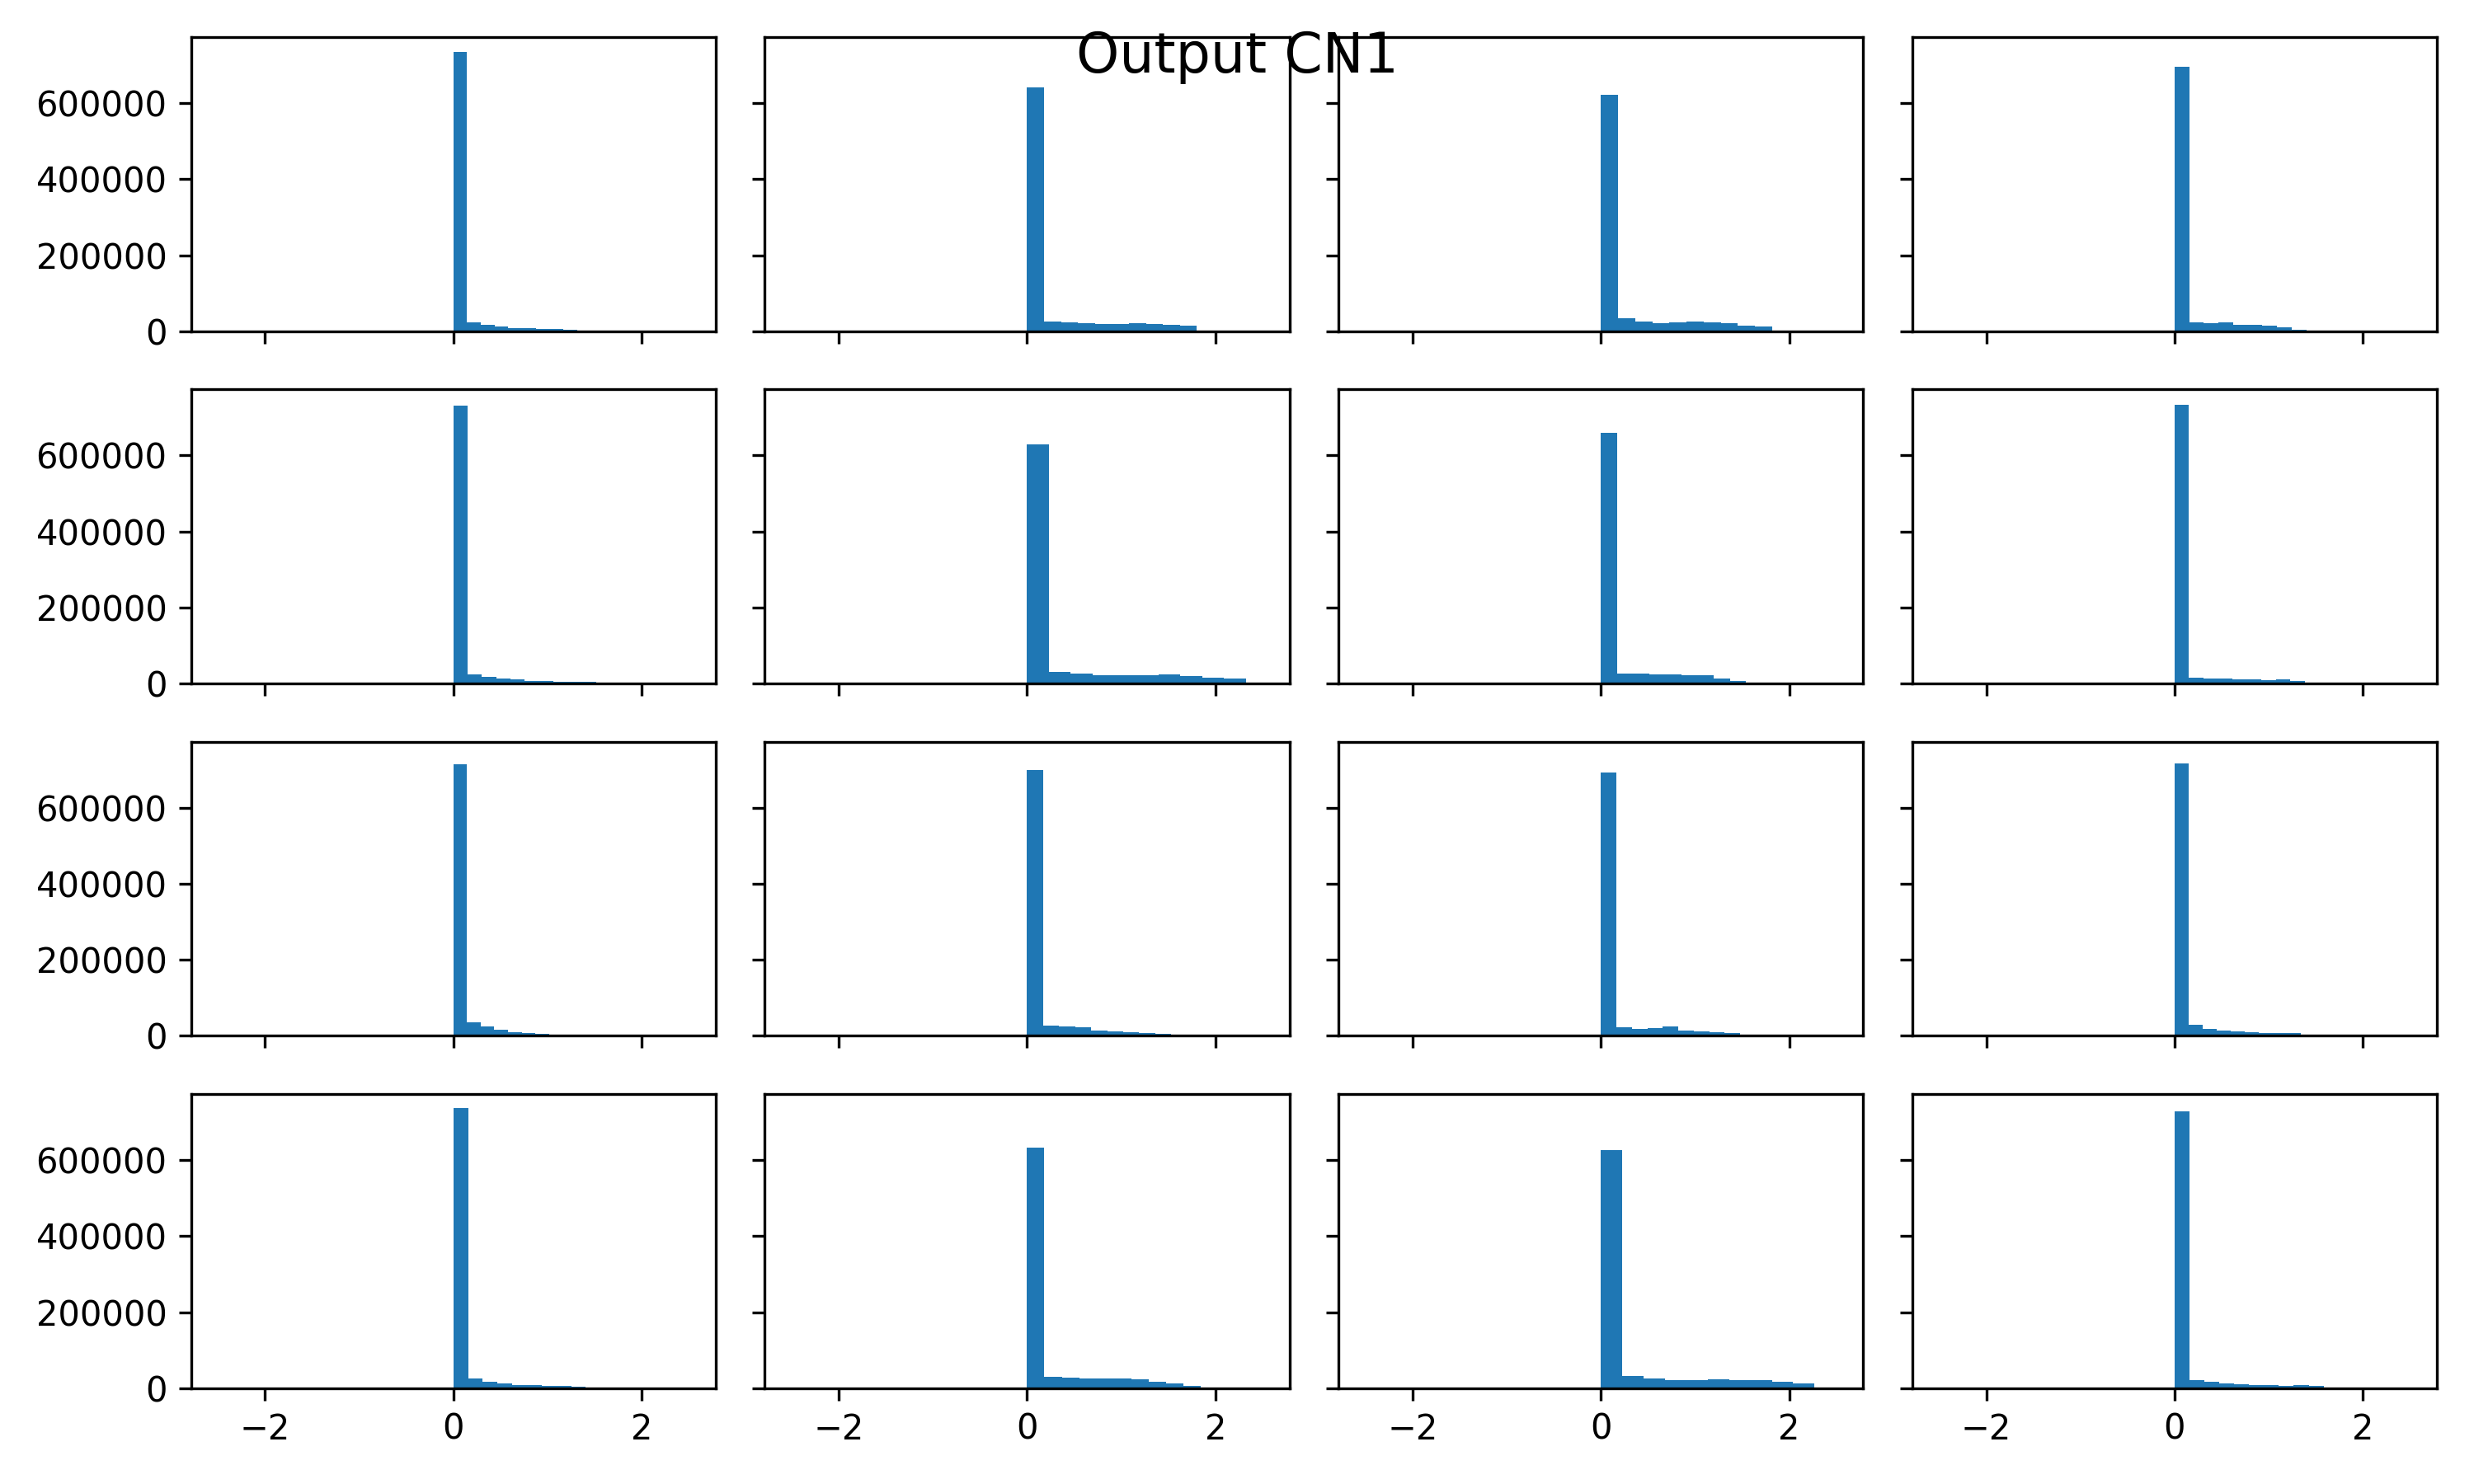
\includegraphics[height=1.6in]{../../net/images/hist_ao1}
        \caption{Convolutional Layer 1}
    \end{subfigure}%
    ~ 
    \begin{subfigure}[t]{0.5\textwidth}
        \centering
         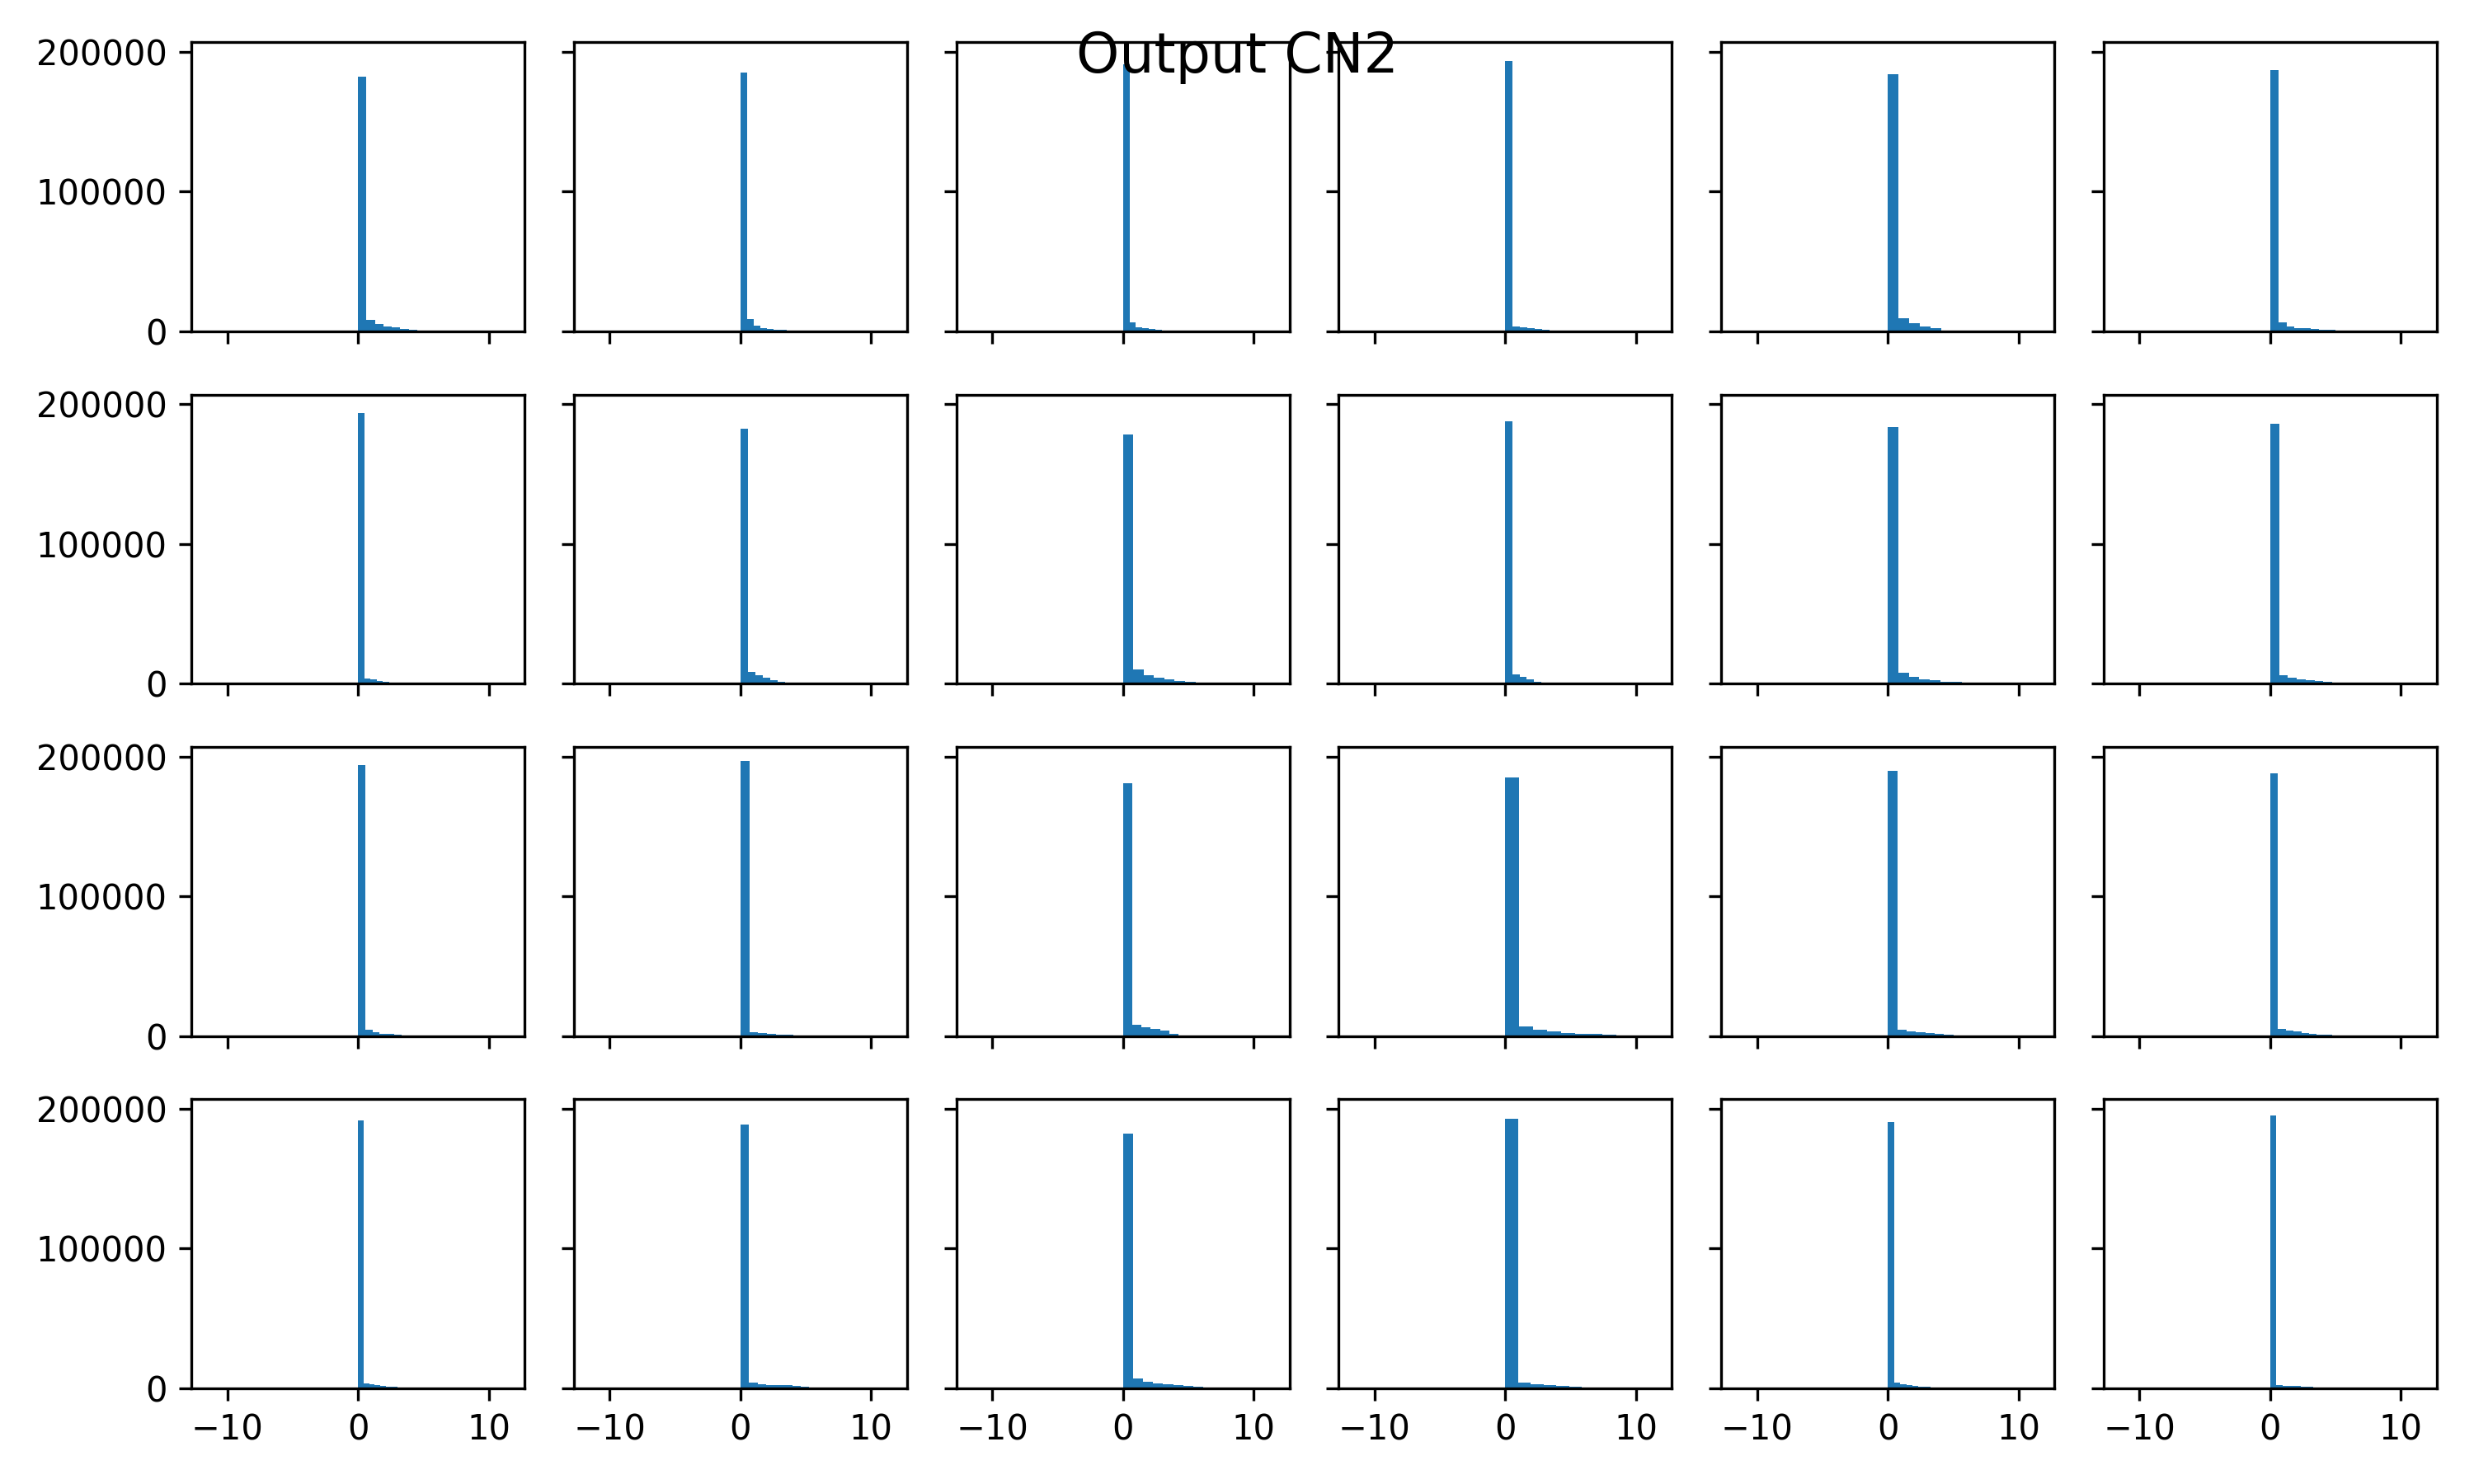
\includegraphics[height=1.6in]{../../net/images/hist_ao2}
        \caption{Convolutional Layer 2}
    \end{subfigure}%
    \\
    \begin{subfigure}[t]{0.5\textwidth}
        \centering
        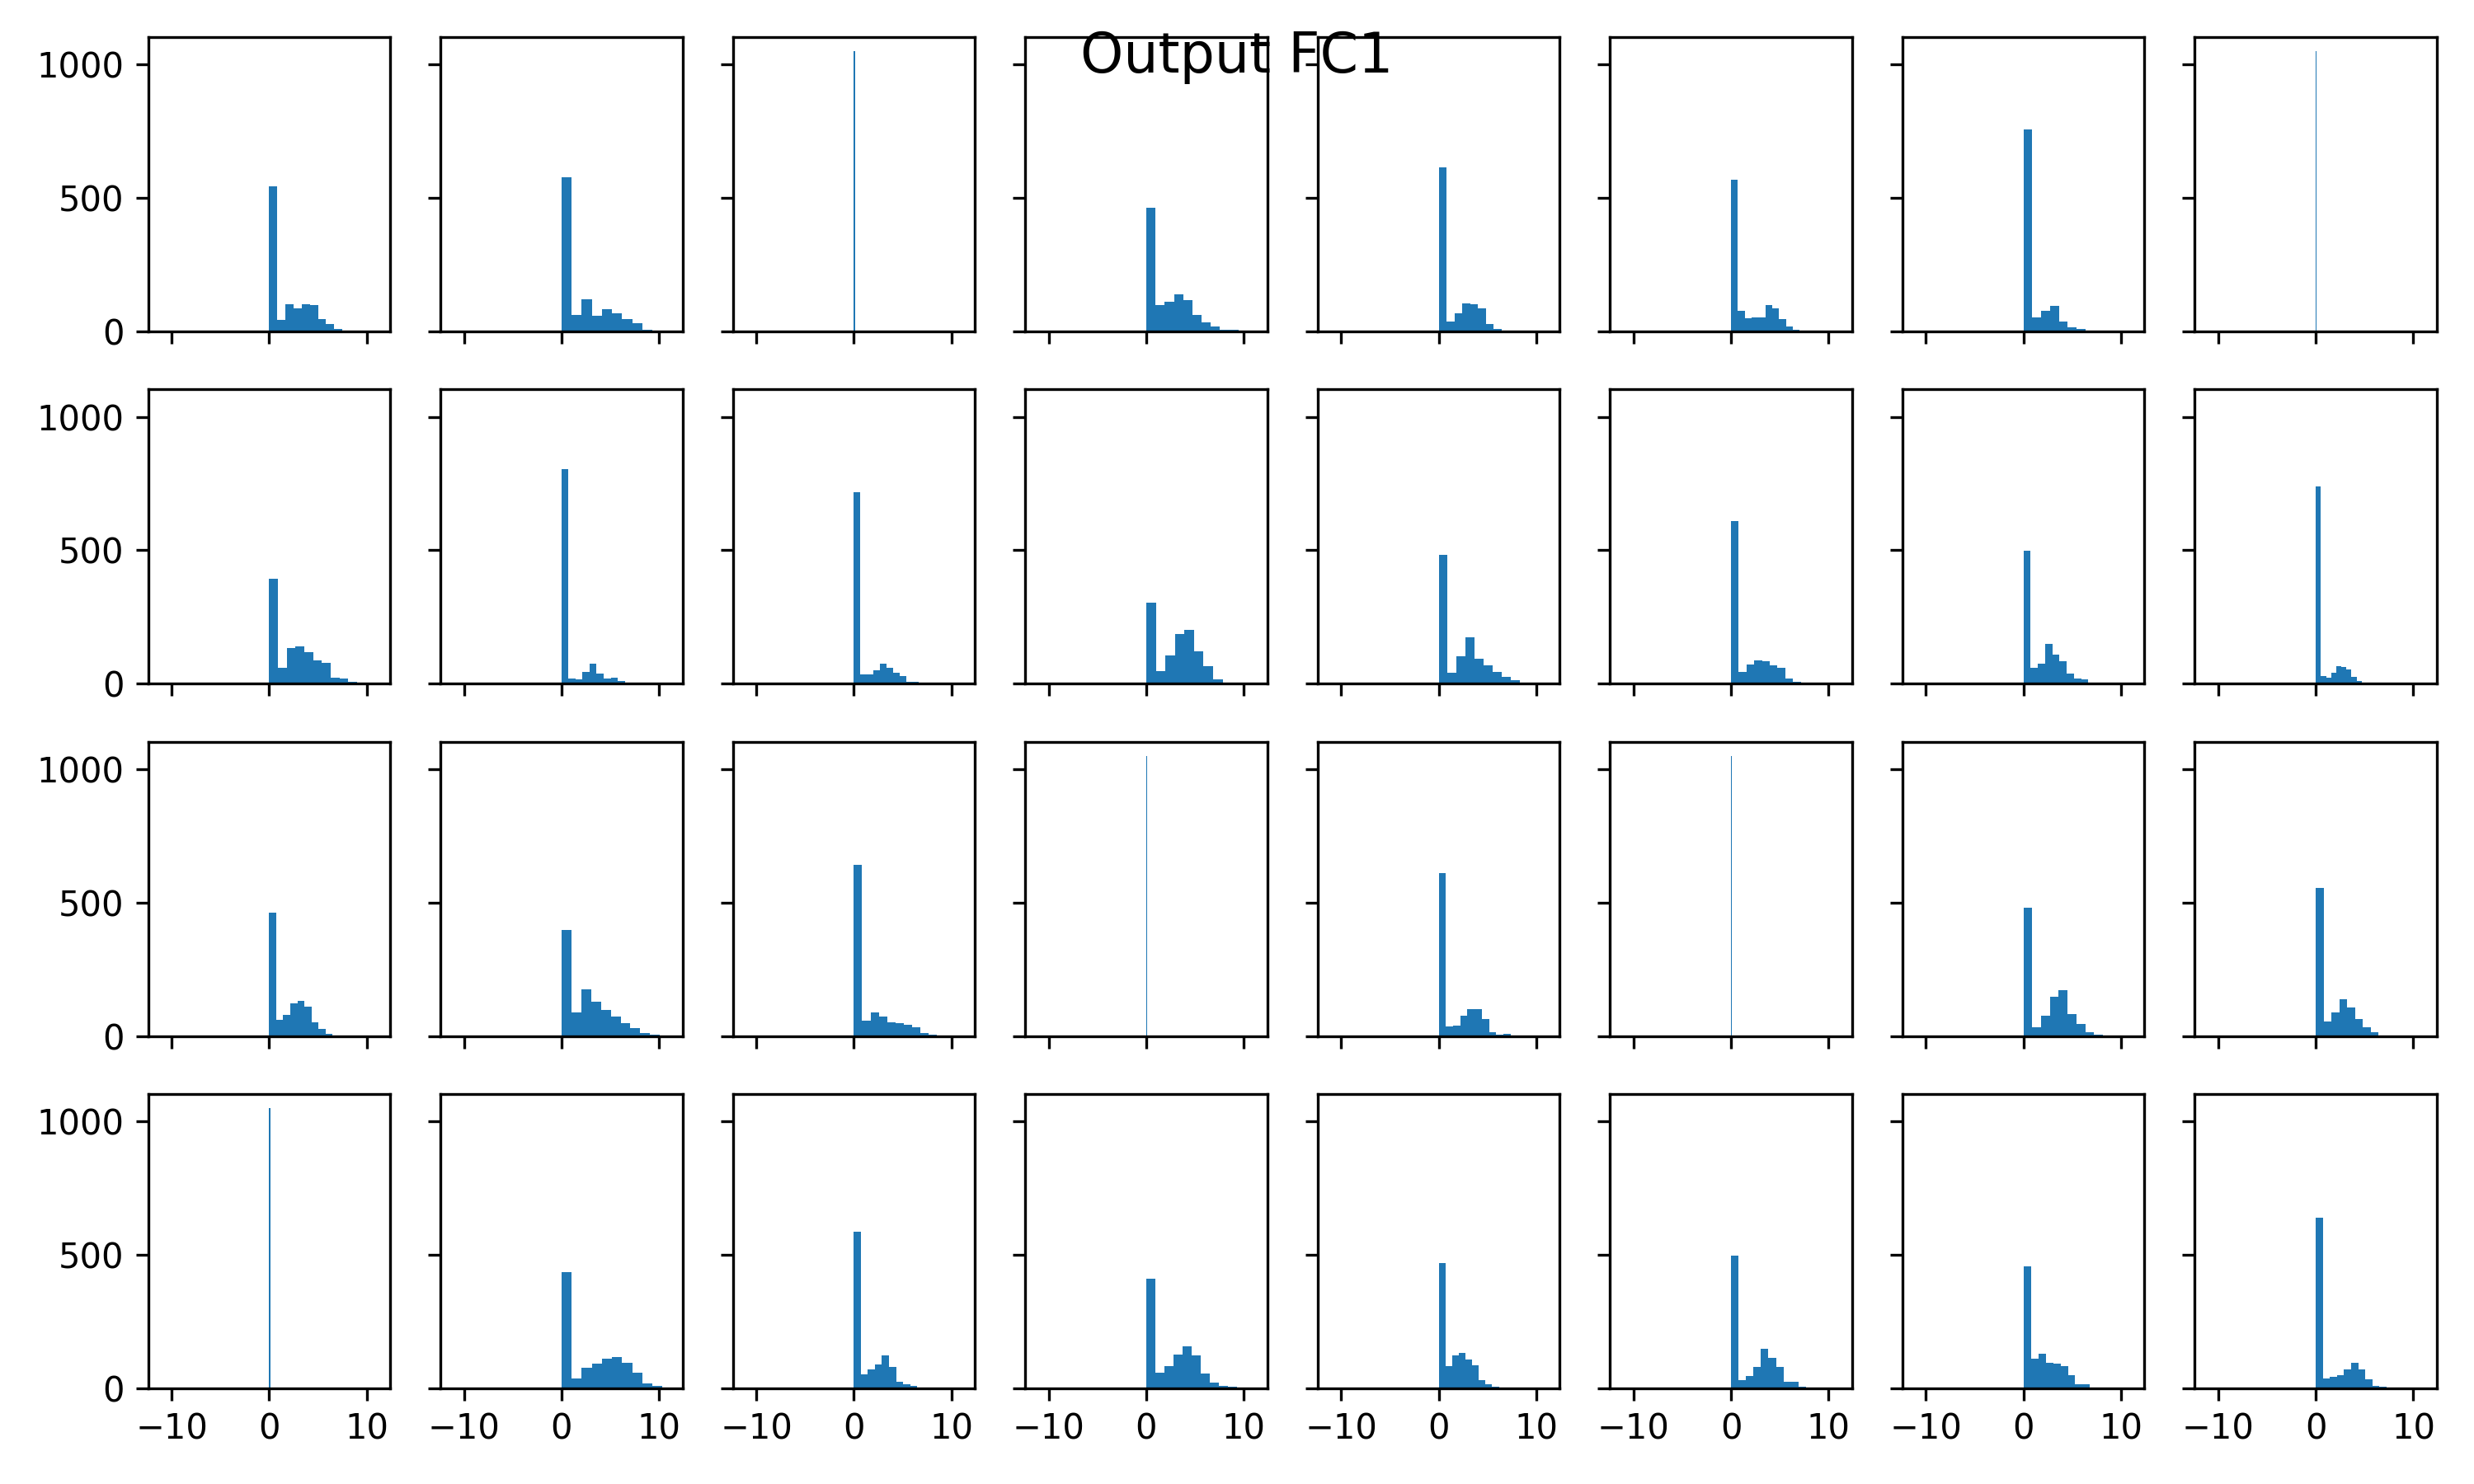
\includegraphics[height=1.6in]{../../net/images/hist_ao3}
        \caption{Fully Connected Layer 1}
    \end{subfigure}%
    ~ 
    \begin{subfigure}[t]{0.5\textwidth}
        \centering
         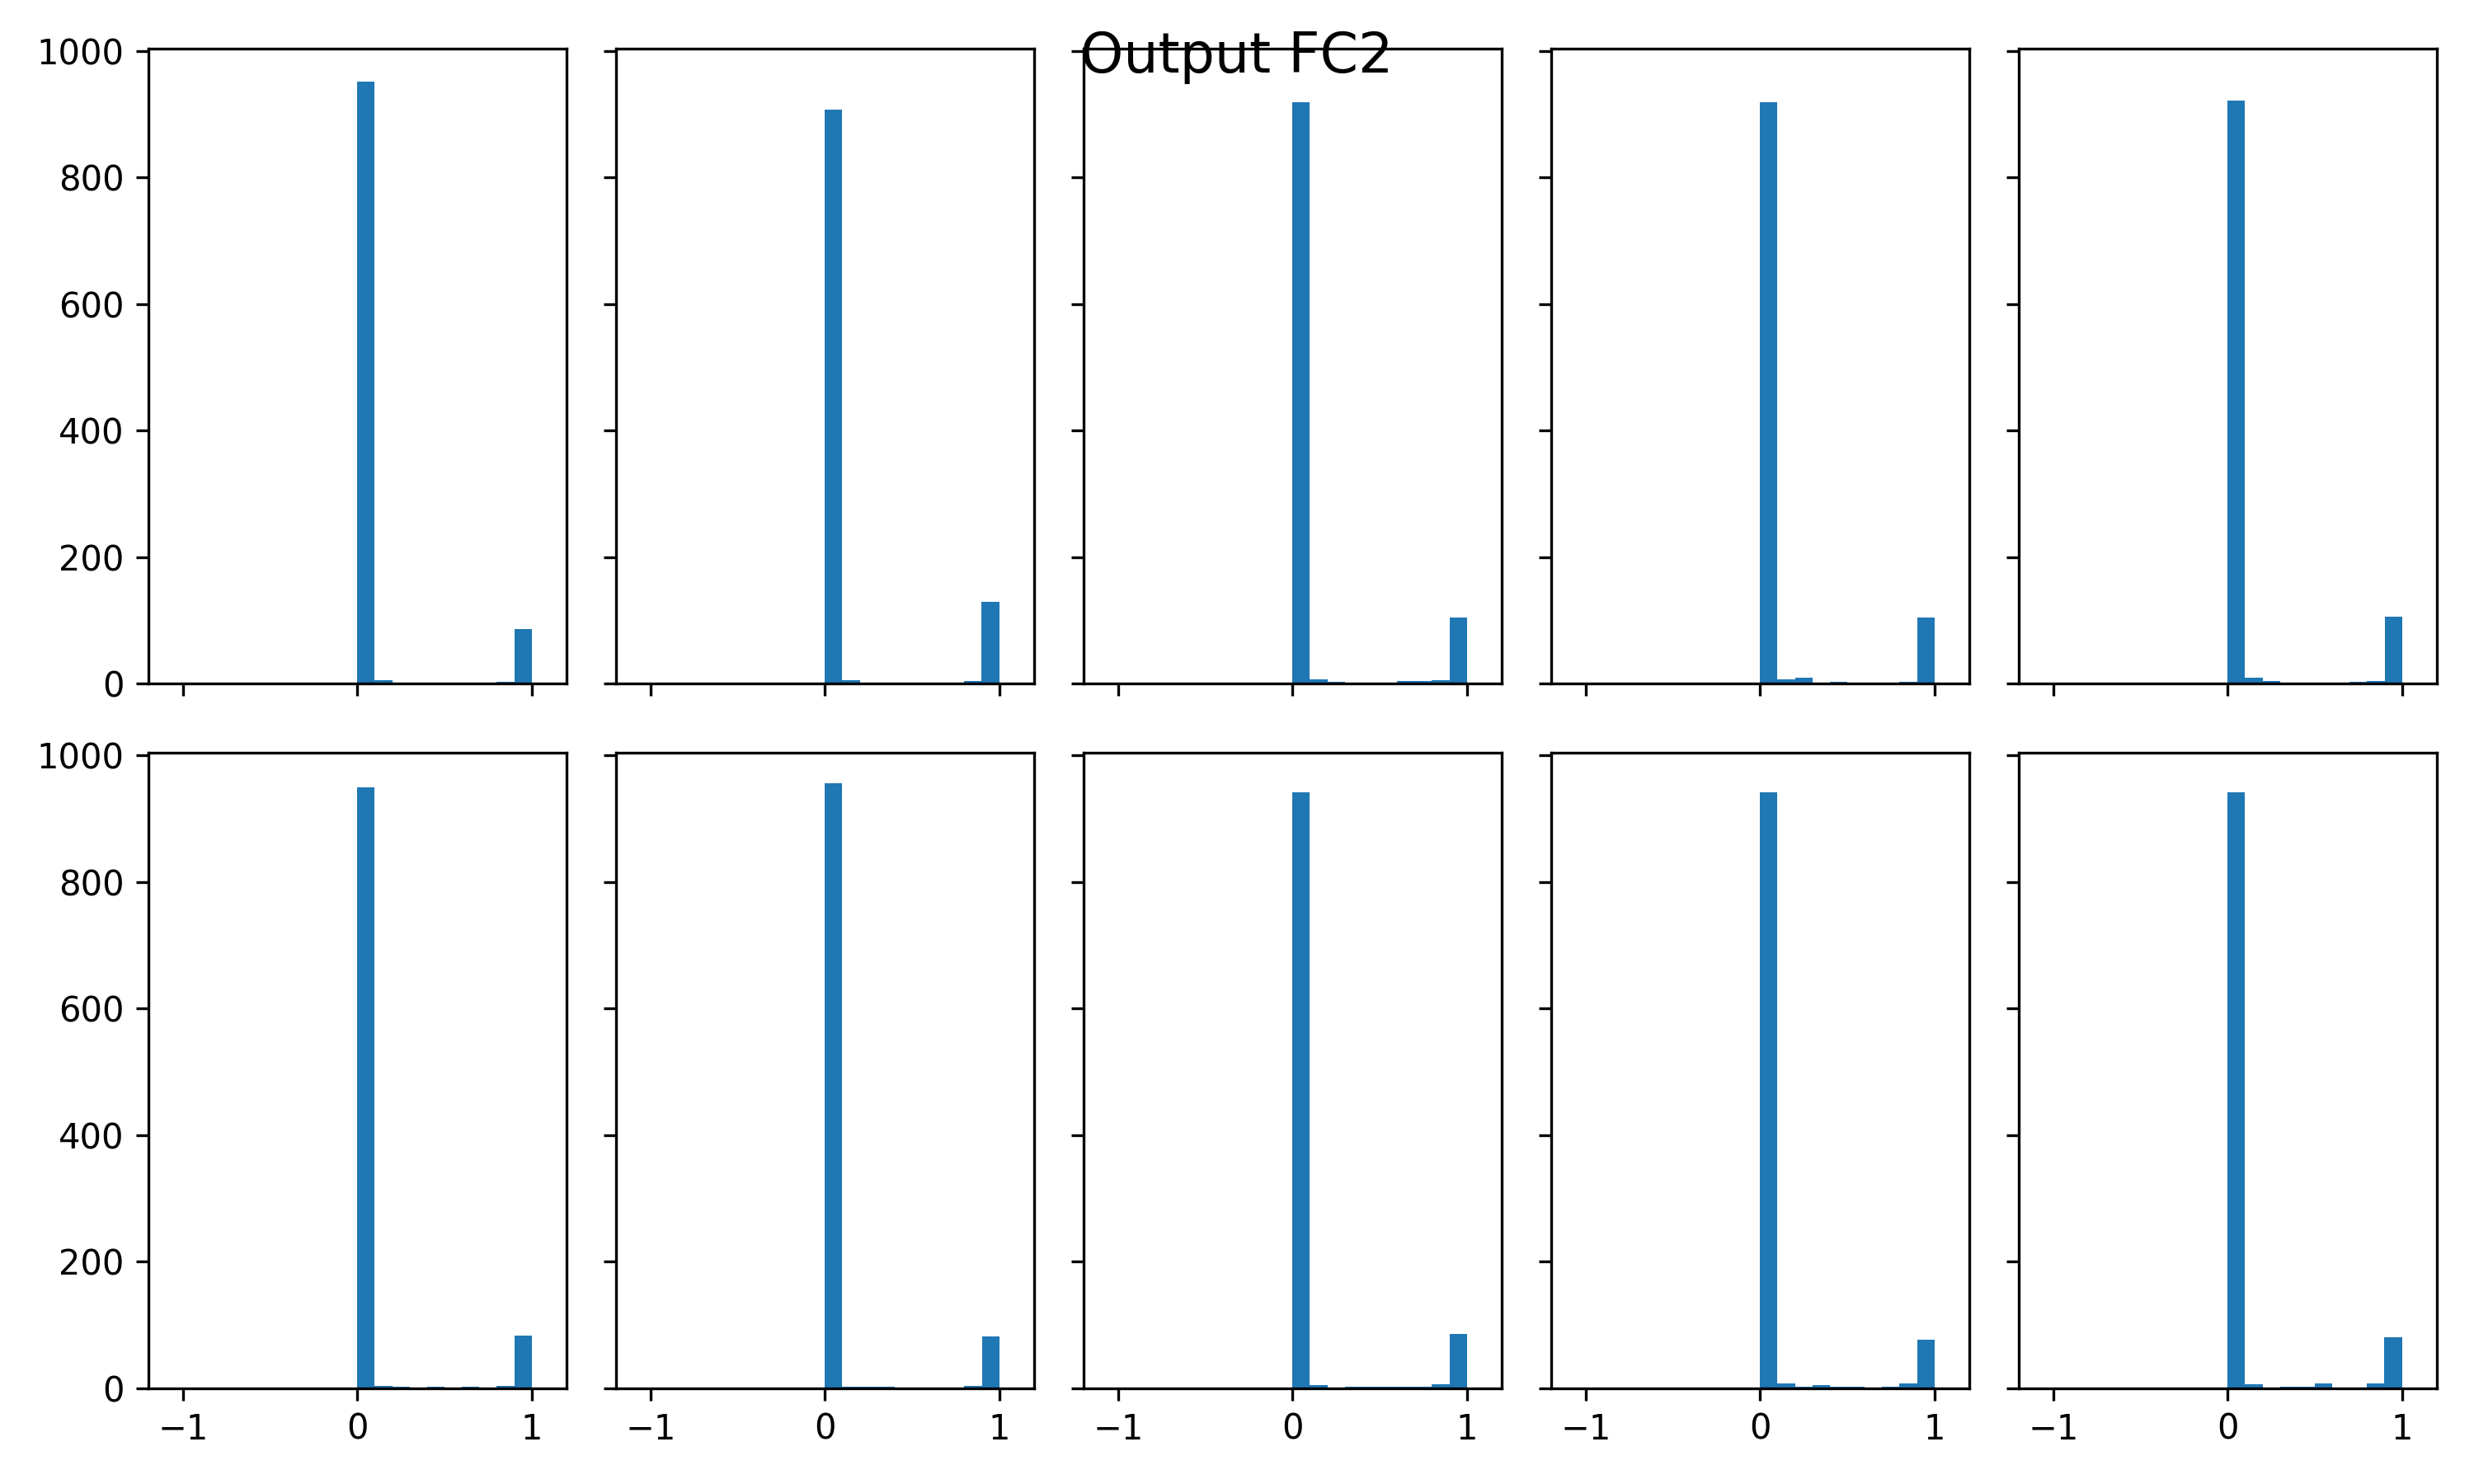
\includegraphics[height=1.6in]{../../net/images/hist_ao4}
        \caption{Fully Connected Layer 2}
    \end{subfigure}
    \caption[Distribution of the activations for a randomly selected batch of the input data]{Distribution of the activations for a randomly selected batch of the input data. The occurring minimum and maximum values were used to define the quantization bit width.}
    \label{fig:network-activations-distributions}
\end{figure}

